\documentclass[conference]{IEEEtran}
\IEEEoverridecommandlockouts
% The preceding line is only needed to identify funding in the first footnote. If that is unneeded, please comment it out.
\usepackage{cite}
\usepackage{amsmath,amssymb,amsfonts}
\usepackage{algorithmic}
\usepackage{float}
\usepackage{graphicx}
\usepackage{textcomp}
\usepackage{xcolor}
\usepackage{hyperref}
\usepackage{subcaption}  %subfigure
\usepackage{multirow}
\usepackage{pgfplots, pgfplotstable}
\pgfplotsset{width=0.45\textwidth, compat=1.9}
\usepgfplotslibrary{external}
\tikzexternalize
\def\BibTeX{{\rm B\kern-.05em{\sc i\kern-.025em b}\kern-.08em
    T\kern-.1667em\lower.7ex\hbox{E}\kern-.125emX}}


    
\begin{document}

\title{Autonomous Drones in Artificial Pollination}

\author{Eric~Lin~\IEEEmembership{(el38),}
        Shaun~Lin~\IEEEmembership{(hl116),}
        and~Karl~Sheng~\IEEEmembership{(ks156)}\\ 
        Advisor: Dr. Joseph Young\\
        Electrical and Computer Engineering, Rice University
        }% <-this % stops a space
\maketitle

\section*{Abstract}
In this report, you'll see the result produced in the spring 2023 semester. As our team, AutoDrone, has equipped drones with computational capability by running a YOLOv5 detection model combined with a MiDaS depth estimation model on the embedded system Jetson Nano 2GB. Using DroneKit and pymavlink libraries, we are able to navigate the drone with Jetson Nano 2GB and/or Raspberry Pi, emulating the behavior of bees. Our tests have shown good precision and agility in visual detection, and we have conducted a successful test flight using a combination of Jetson Nano 2GB and/or Raspberry Pi with a drone. Our results demonstrate the feasibility of using autonomous drones for artificial pollination and resolving the shortage of pollinators. \\

Keywords: Autonomous Drone, Drone Navigation, Artificial Pollination, YOLOv5, Object Detection, MiDaS, Depth Estimation, Flower Detection, Jetson Series, Raspberry Pi.

% \begin{IEEEkeywords}
% autonomous drone, artificial pollination, YOLOv5, MiDaS, Jetson Series, SITL, Raspberry Pi
% \end{IEEEkeywords}


\section{Introduction}
Bees are essential for pollinating crops and flowers, but their populations are declining rapidly. According to Bee Informed Partnership, an estimated 32.2\% of managed colonies in the United State lost during the winter of 2020-2021 \cite{b1}, and Food and Agriculture Organization of United Nations report that global losses of 10-15\% each year, with some countries reporting losses of up to 30\% \cite{b2}. To address this problem, there are researchers investigating small insect-like flying robots with remote control \cite{b3}, which shows the possibility to make it autonomous.

Additionally, another previous robotic pollination researches \cite{b4}, developed an precision robotic pollination system, they focused on localization and mapping, visual perception, path planning and motion control, the system is based on a ground-based robotic arm for pollination tasks, and the system is unable to handle high sensitivity and tackle complex terrain areas for pollination tasks as well as a real bee.

Therefore, this project aims to explore the use of a flying drone for pollination. Robotic pollinators, such as autonomous drones, have the potential to revolutionize the future of pollination and agriculture, using low-cost camera-based sensors and deep learning technology to develop an effective and sustainable solution with drones to address the problem of declining honeybee populations and their impact on food production.
\section{Methods}

\subsection{Hardware}\label{subsection:A}
This section contains all hardware used in this capstone project.
    \subsubsection{Drone Kit}\label{subsection:A1}
    \begin{itemize}
        \item QWinOut Q705 6-Aixs RC Drone
        \item QWinOut J630 4-Aixs RC Drone
    \end{itemize}

    \begin{figure}[H]
        \centerline{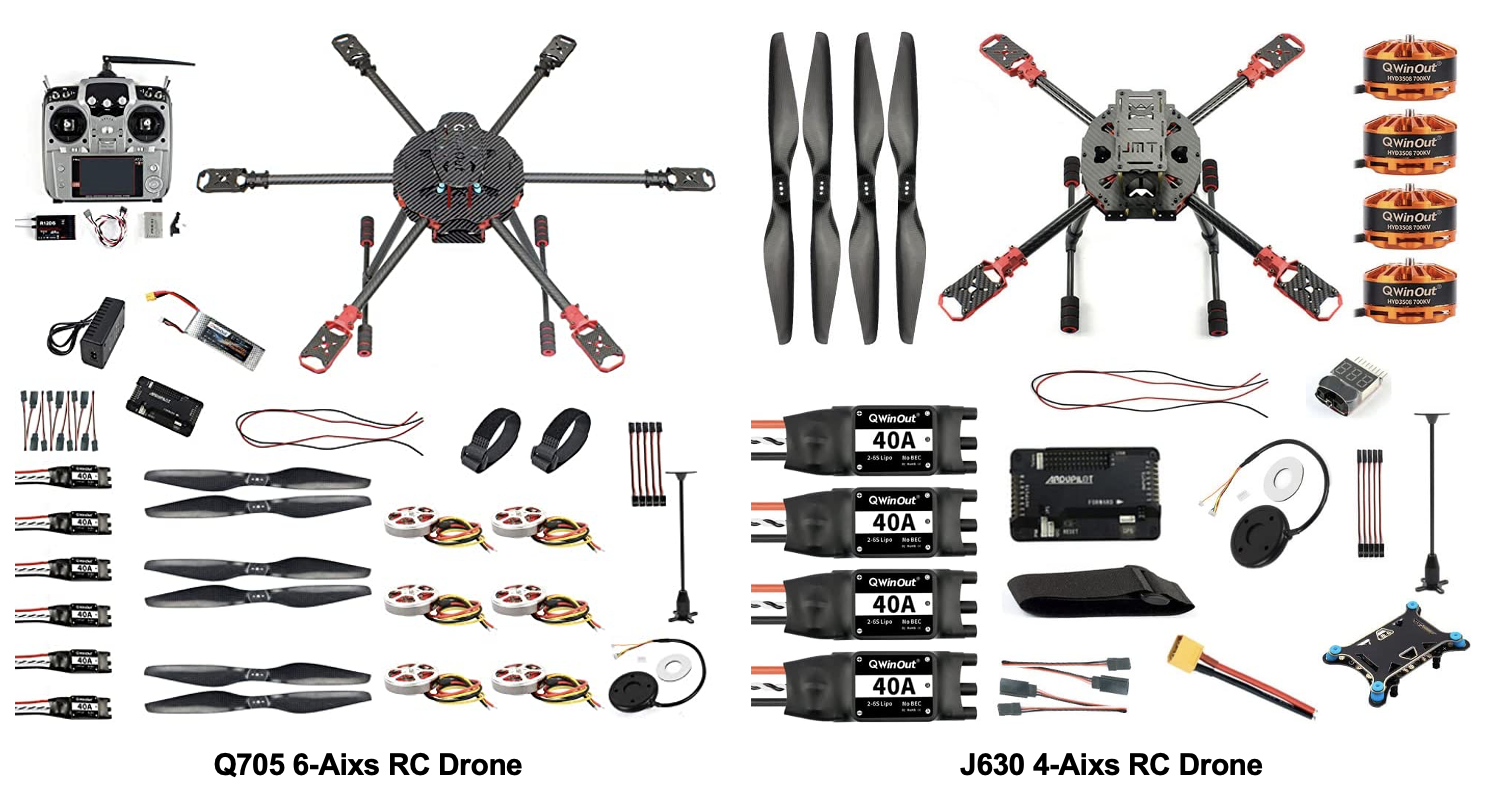
\includegraphics[width=0.5\textwidth]{Figures/Methods/Drone_Kits.png}}
        \caption{(left) 6-Axis RC Drone / (right) 4-Axis RC Drone.}
        \label{fig1}
    \end{figure}
    
    There are two types of drones used in the project, as shown in Fig.~\ref{fig1}, the larger 6-axis RC drone and the new smaller 4-axis drone purchased this 2023 spring semester. The larger 6-axis drone is a continuation of the team's work from last semester, and the smaller 4-axis drone is a new drone that we assembled this semester.
    
    \subsubsection{Transistor \& Receiver}\label{subsection:A2}
    \begin{itemize}
        \item SIK Telemetry Radio
        \item Flysky FS-i6   6CH 2.4GHz RC Transmitter
        \item Flysky FS-i6X 10CH 2.4GHz RC Transmitter
        \item iA6B Receiver
        \item iA10B Receiver
    \end{itemize}

    \begin{figure}[H]
        \centerline{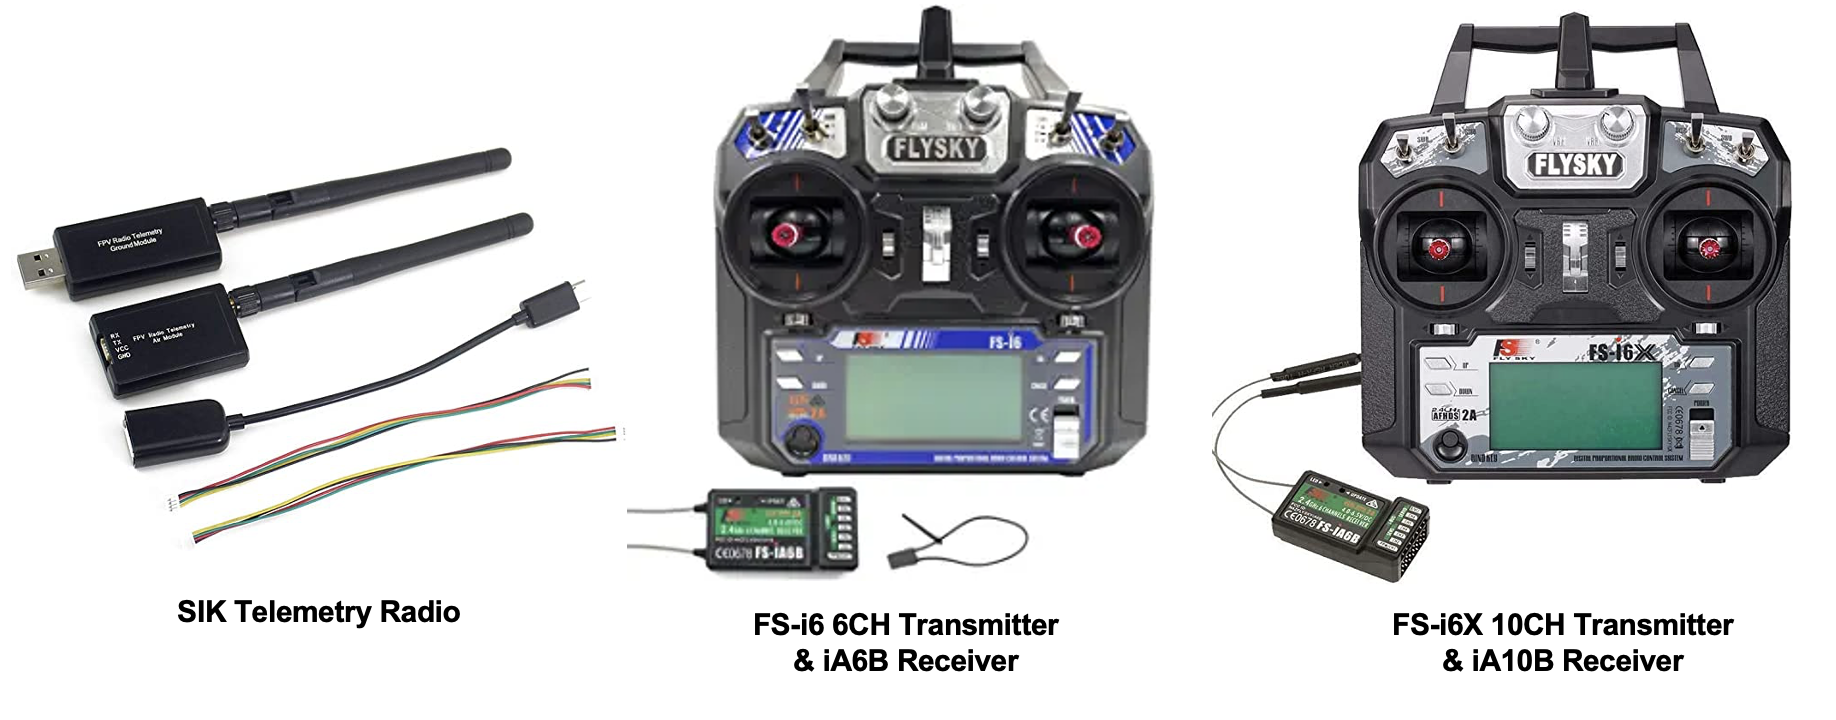
\includegraphics[width=0.5\textwidth]{Figures/Methods/Transistors&Receivers.png}}
        \caption{(left) SIK Telemetry Radio / (middle) FS-i6 6CH Transmitter \& iA6B Receiver / (right) FS-i6X 10CH Transmitter \& iA10B Receiver.}
        \label{fig2}
    \end{figure}

    Since we use two types of drones, there are different Transistors \& Receivers for each, as shown in Fig.~\ref{fig2}. FS-i6 6CH and iA6B Receiver pairing is for 6-axis drone. FS-i6X 10CH and iA10B Receiver pairing is for 4-axis drone. Then SIK radio just used to communicate between flight controller and Laptop/PC.
    
    \subsubsection{Flight Controller}\label{subsection:A3}
    \begin{itemize}
        \item Cube Black Flight Controller
        \item APM2.8 Flight Controller
    \end{itemize}

    \begin{figure}[H]
        \centerline{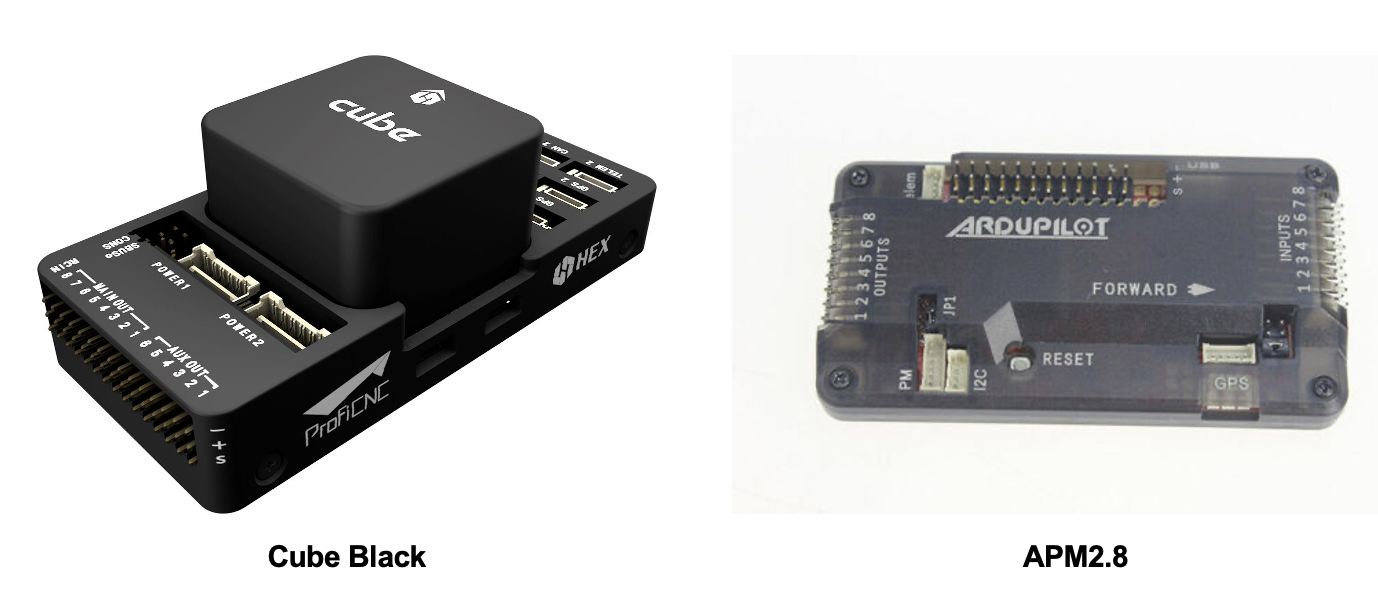
\includegraphics[width=0.5\textwidth]{Figures/Methods/Flight_Controllers.png}}
        \caption{(left) Cube Black / (right) APM2.8.}
        \label{fig3}
    \end{figure}

    Flight controller plays one of the crucial roles in this project, as it is responsible for controlling the drone's flight and stability. It receives sensor data from various sensors and makes necessary adjustments to maintain the desired altitude, orientation, and movement of the drone. It's including an accelerometer, gyroscope, magnetometer, and barometer.

    We used two flight controller modules that came with the Drone Kit in this project, as shown in Fig.~\ref{fig3}, so that we could expedite our development and spend more time on Deep Learning algorithms.
    
    \subsubsection{Embedded System / Controller}\label{subsection:A4}
    \begin{itemize}
        \item Jetson Nano 2GB
        \item Raspberry Pi 3B
        \item Raspberry Pi 4B
    \end{itemize}

     \begin{figure}[H]
        \centerline{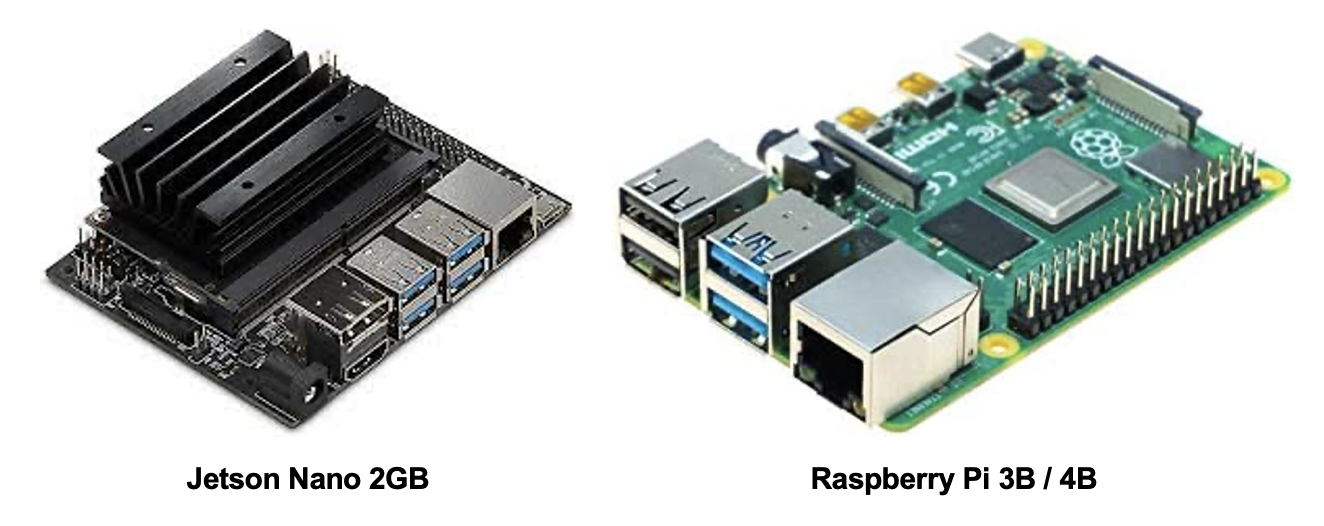
\includegraphics[width=0.5\textwidth]{Figures/Methods/Embedded_Systems.png}}
        \caption{(left) Jetson Nano 2GB / (right) Raspberry Pi 3B / 4B.}
        \label{fig4}
    \end{figure}

    The embedded system is the main controller in the system, which plays a critical role in performing all the tasks. It collects images from the camera sensor and uses deep learning algorithms to correctly identify flower types, track flower locations and calculate depth information, and then sends commands to the flight controller to precisely control the drone to successfully complete the artificial pollination task.

    Here we use two types of embedded devices, as shown in Fig.~\ref{fig4}, the Jetson Nano 2GB with built-in GPU and the smaller Raspberry Pi 3B / 4B. We will test these two types of embedded devices and compare which one is more compatible for the project.

\subsection{System Design}\label{subsection:B}

The system consists of essential components, including a Jetson Nano 2GB and/or Raspberry Pi to process deep learning models. The Drone-Kit API and MAVLink protocol facilitate communication with the Cube Black flight controller, which ultimately controls the drone's motor and navigation. The system flow chart is depicted in Fig.~\ref{fig5}.

Two embedded devices, the Jetson Nano and Raspberry Pi, are incorporated into the drone to compare their performance. Additionally, a SIK radio block is utilized to send the drone's status back to a Laptop/PC for real-time monitoring. For added safety, a Flysky FS-i6 6CH 2.4GHz RC Transmitter and iA6B Receiver are included to enable manual drone control.

    \begin{figure}[H]
        \centerline{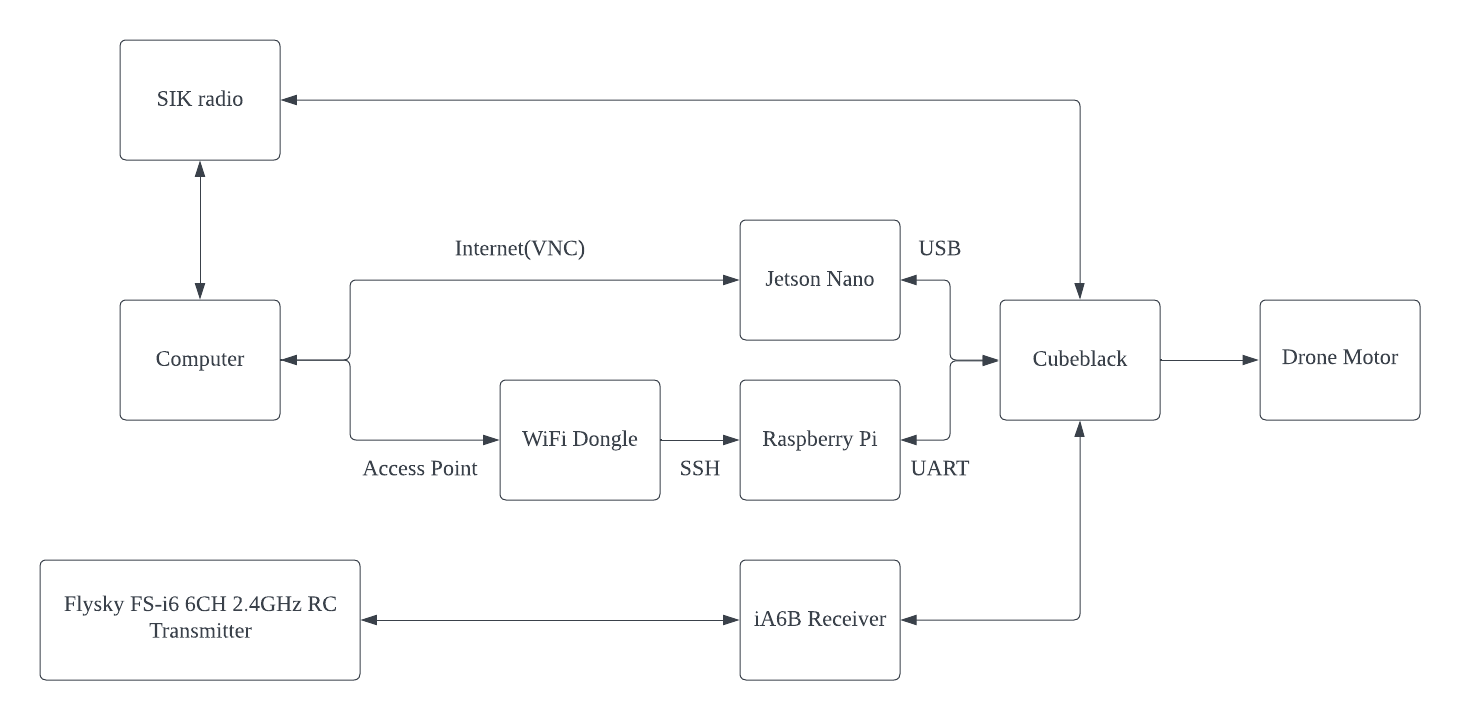
\includegraphics[width=0.5\textwidth]{Figures/Methods/System Flow Chart.png}}
        \caption{System Flow Chart.}
        \label{fig5}
    \end{figure}

    \begin{figure}[H]
        \centerline{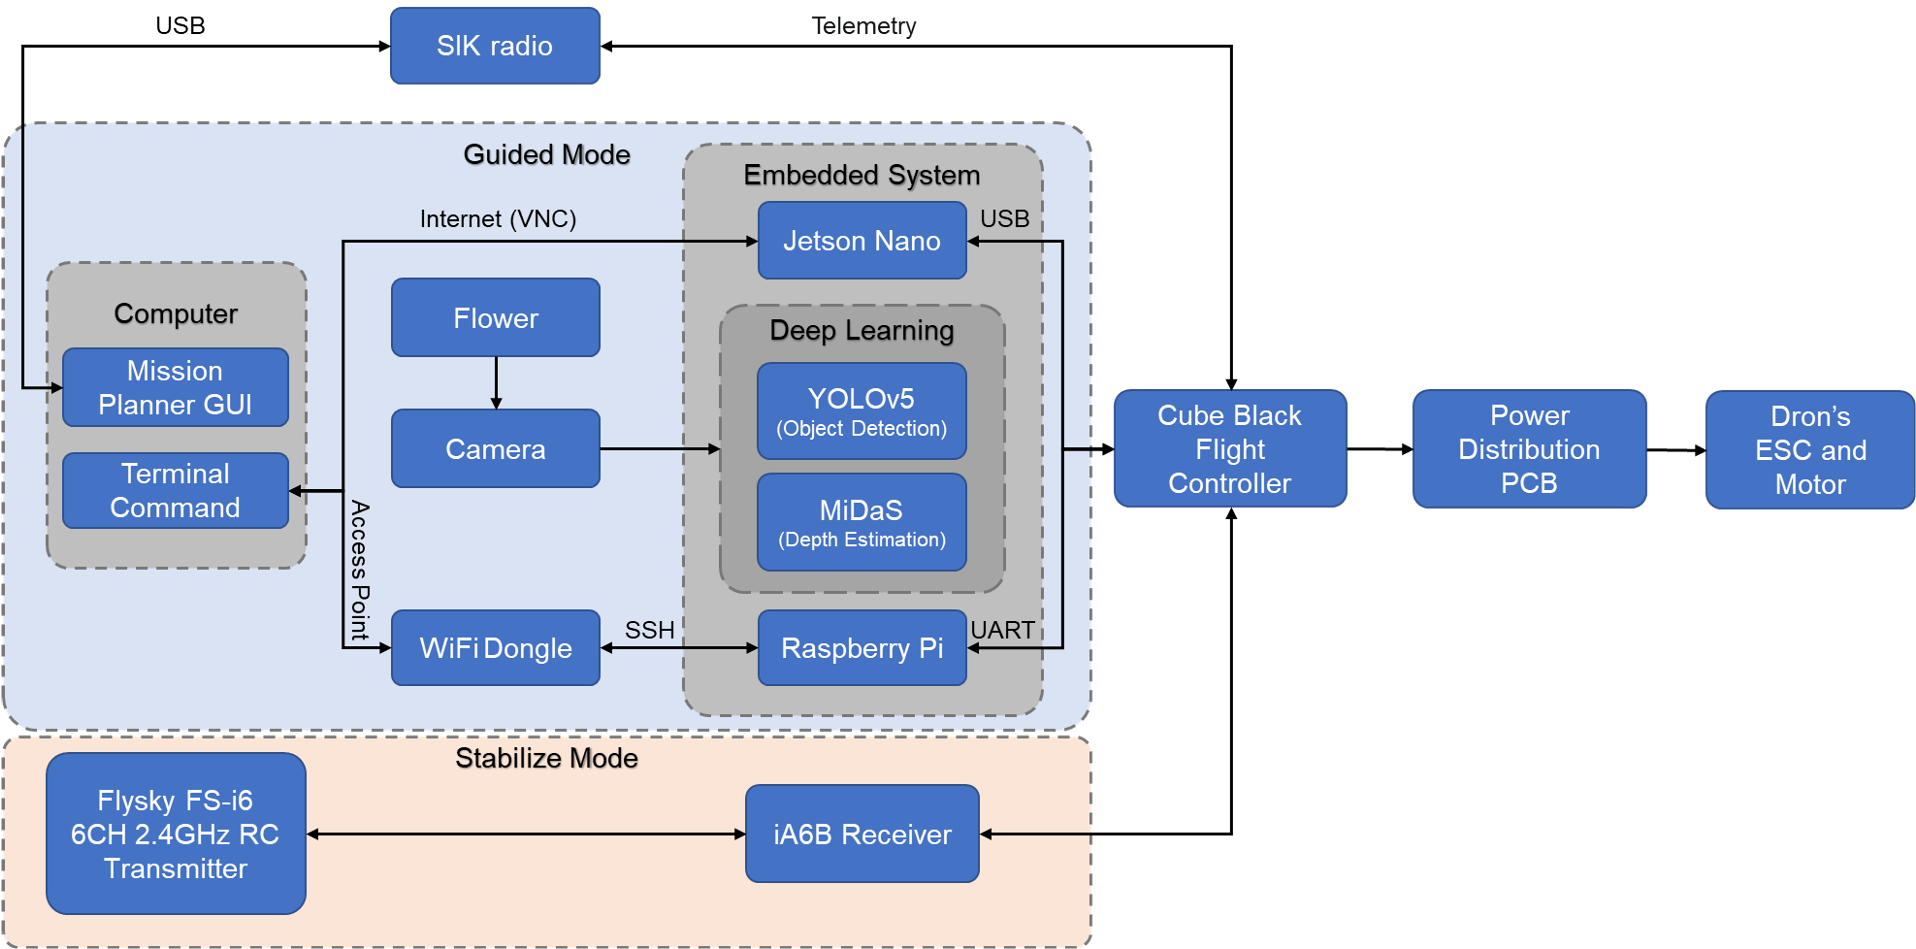
\includegraphics[width=0.5\textwidth]{Figures/Methods/System_Overall_Design.png}}
        \caption{Overall System Design.}
        \label{fig6}
    \end{figure}

Fig.~\ref{fig6} provides a detailed overview of the system design. The process starts with capturing an image of a flower using a camera sensor. The image is then analyzed using Deep Learning's YOLOv5 object detection model and MiDaS depth estimation model, both of which run on the Embedded System Jetson Nano 2GB and/or Raspberry Pi. YOLOv5 is used to detect flowers in the image (Please note sections \ref{subsection:C} below for more information on YOLOv5), while MiDaS calculates the distance between the flowers and the drone. (Please note sections \ref{subsection:D} below for more information on MiDaS)

 For manual control, we use the Flysky FS-i6 6CH 2.4GHz RC Transmitter in Stabilize Mode, which disables pre-arming checking and puts the drone in an unstable mode. However, to operate the drone using scripts, it must be set to Guided Mode, which allows pre-arming checks to ensure the drone is in a safe condition to complete the pollination task.
    
\subsection{YOLOv5}\label{subsection:C}

Object detection is a crucial aspect of autonomous drone operation. While there are many deep learning models that can be used for flower detection, Convolutional Neural Networks (CNNs) are the most researched method \cite{b5, b6}. However, these models mostly use a two-stage pipeline which may not be efficient for autonomous drone purposes. In contrast, one-stage models such as YOLO (You Only Look Once) \cite{b7} model is a state-of-the-art real-time object detection algorithm, known for its high speed and accuracy. YOLO processes the input image by dividing it into a grid and predicting a set of bounding boxes, objectness scores, and class probabilities for each grid cell. These predictions are combined and subjected to non-maximum suppression to remove overlapping boxes, generating the final object detections.

In our autonomous drone pollination project, the primary objective is to detect flowers using a webcam mounted on the drone. The YOLO model plays a crucial role in identifying flowers within the camera frame. We utilized the YOLOv5 architecture \cite{b8} for this project, which is an enhanced version of the original YOLO model. YOLOv5 is implemented in the PyTorch framework and offers a range of pre-trained models, each with different trade-offs between speed and accuracy. Given the limited computational resources available on drones, we chose the smaller YOLOv5 model, YOLOv5s, which has only 7.2 million parameters.

In addition to the model trained by the Ultralytics team, we also investigated the methods employed by the previous Autodrone team. They incorporated knowledge distillation \cite{b9} into the original YOLOv5 training framework, a technique that transfers knowledge from a larger model to a smaller model, thereby enhancing the performance of the smaller model. A larger model served as a teacher model, with its output functioning as a soft label to instruct the student model.

By leveraging the efficient YOLOv5s architecture and incorporating knowledge distillation, our flower detection model achieves high accuracy while maintaining real-time performance, making it suitable for deployment on resource-constrained platforms such as drones. This combination of techniques enables the autonomous drone pollination system to effectively detect flowers or other objects in real-world environments, thus constructing a key foundation for the autonomous pollination system.

\subsection{MiDaS}\label{subsection:D}

To accurately estimate the distance of flowers from the drone, we employed the MiDaS (Monocular Depth Estimation of High Resolution Images with Pyramid Stereo Fusion) model \cite{b10}. The MiDaS model is a state-of-the-art depth estimation algorithm known for its speed and accuracy. It can estimate depth from a single image without the need for stereo cameras. The model utilizes a deep neural network to learn a mapping between the input image and its corresponding depth map, which is subsequently used to calculate the distance of the flower from the drone.

While there are alternative methods to determine the distance between objects and the camera with higher accuracy, such as stereo vision, these approaches tend to consume more computing resources and power. Given the constraints of the embedded system on the drone, we opted to use the MiDaS depth estimation model based on a monocular camera. Theoretically speaking, this model allows us to estimate the depth of the flower using a single image captured by the drone, reducing computational requirements and power consumption while still providing reliable depth estimation.

The MiDaS depth map estimates the depth of each pixel in an input image, representing the distance of that pixel from the camera. However, several factors can affect the accuracy of the depth map, including the quality of the input image, the distance of the object from the camera, and the lighting conditions. To evaluate the performance of the MiDaS model and assess its suitability for depth estimation on a drone, we conducted two experiments aimed at determining the numerical relationship between the depth map intensity and the real-world distance in meters.

The first experiment was set up inside the ECE lab, as illustrated in Fig. ~\ref{fig7}. Multiple tapes were placed on the floor at 1-meter intervals. The camera was positioned steadily at the 0-meter line. In this controlled environment, chairs were placed on the marked lines and served as detected objects.

\begin{figure}[H]
    \centerline{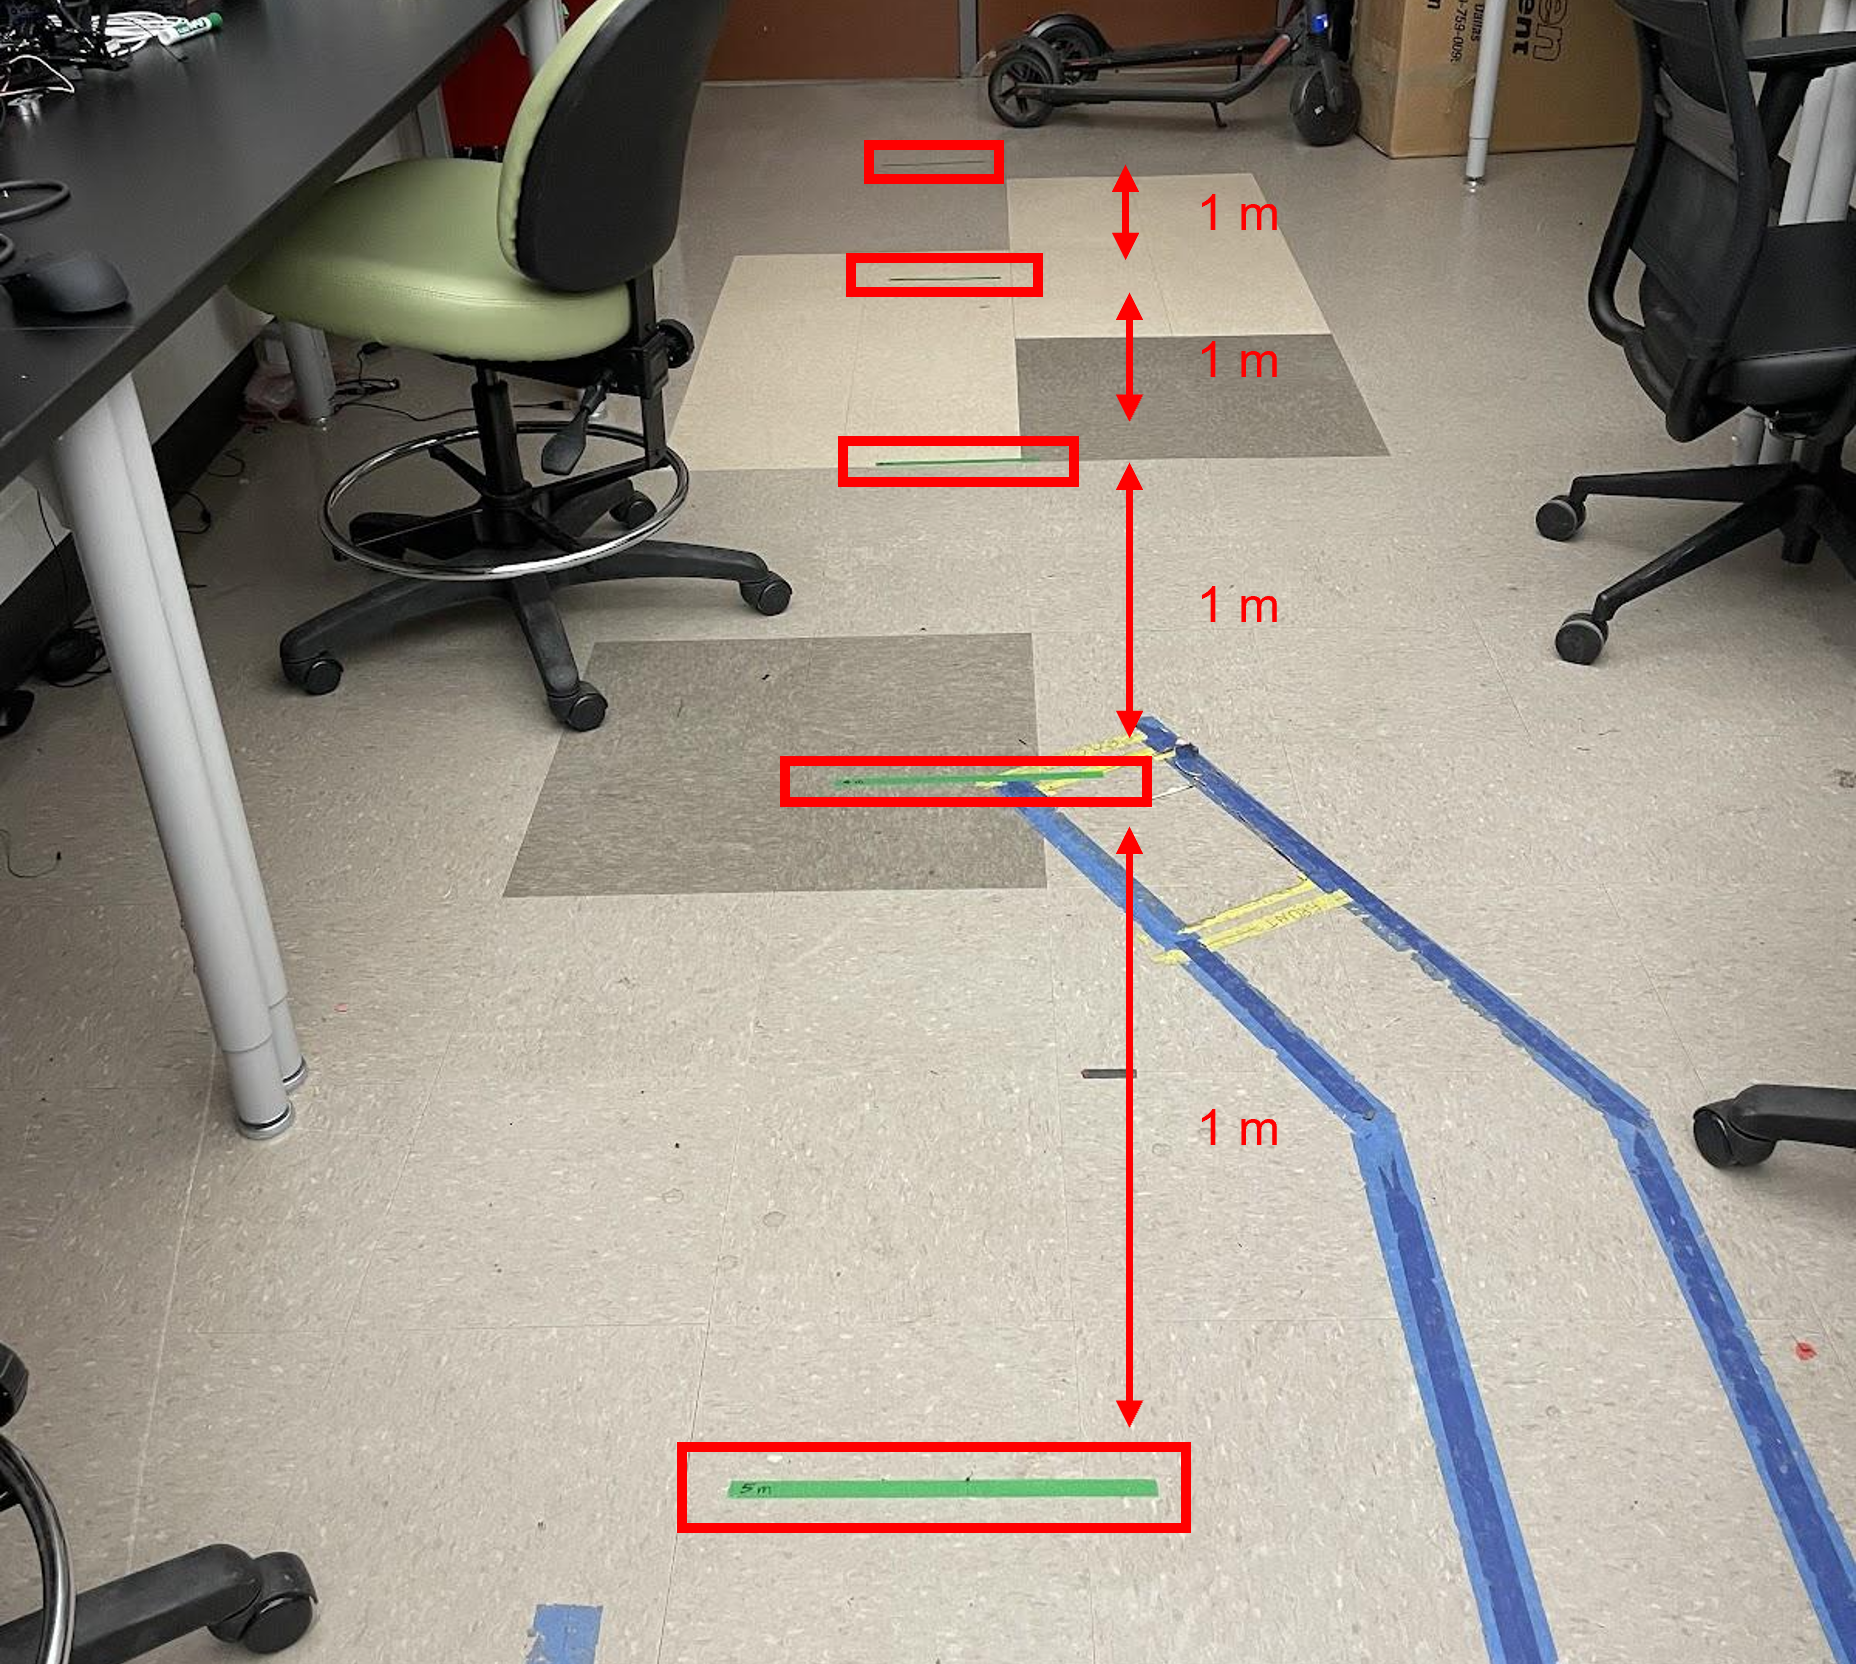
\includegraphics[width=0.5\textwidth]{Figures/Methods/env1.png}}
    \caption{Indoor Environment of the First Experiment}
    \label{fig7}
\end{figure}

    
The second experiment was conducted outdoors in an open environment, as shown in Fig. ~\ref{fig8.1}. The objective was to simulate object detection and depth estimation in a real autonomous pollination task with noise and unexpected anomalies occurring in the camera frame within a dynamic environment. The experiment involved a webcam mounted onto the drone, a team member carrying the drone and holding one end of a tape measure, and another team member holding the other end of the tape measure, acting as the detected object, and recording the actual distances from the camera. This experiment was performed twice from two different orientations to test whether the orientation of sunlight was another contributing factor to the depth map intensity.


\begin{figure}[H]
    \centerline{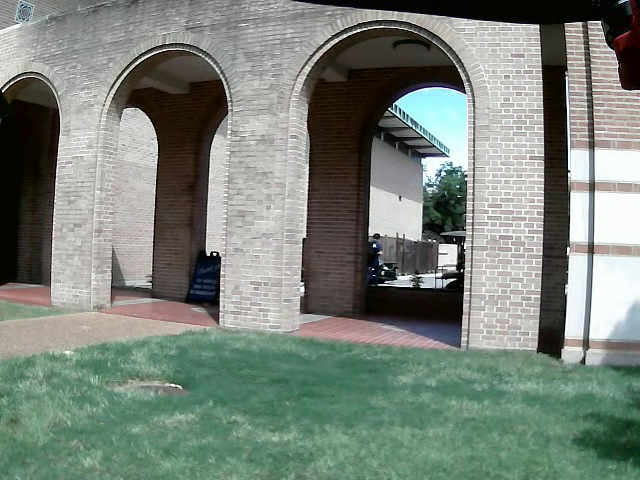
\includegraphics[width=0.5\textwidth]{Figures/Methods/env2a.png}}
    \label{fig8.1}
\end{figure}

\begin{figure}[H]
    \centerline{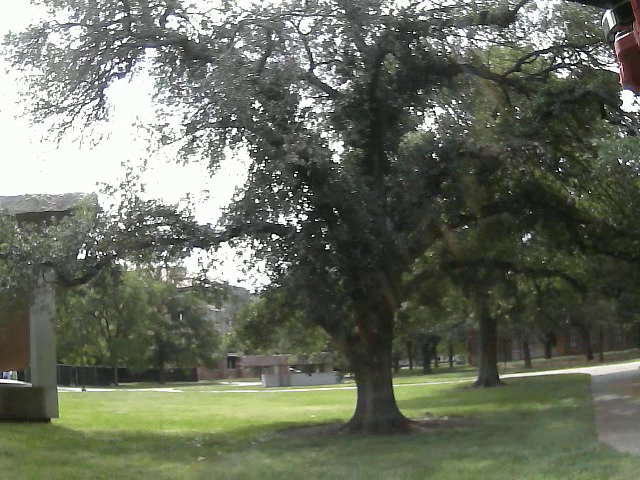
\includegraphics[width=0.5\textwidth]{Figures/Methods/env2b.png}}
    \caption{Outdoor Environments of the Second Experiment}
    \label{fig8.2}
\end{figure}

The results and interpretation of these experiments will be elaborated in detail in the following Results subsection.

\subsection{UI}\label{subsection:E}
To monitor the drone's status in real-time, we utilize the SIK Telemetry Radio and Mission Planner GUI. This eliminates the need to develop a complex GUI interface and provides detailed drone status information.
\section{Results}

\subsection{Raspberry Pi Integration}

\begin{figure}[H]
    \centerline{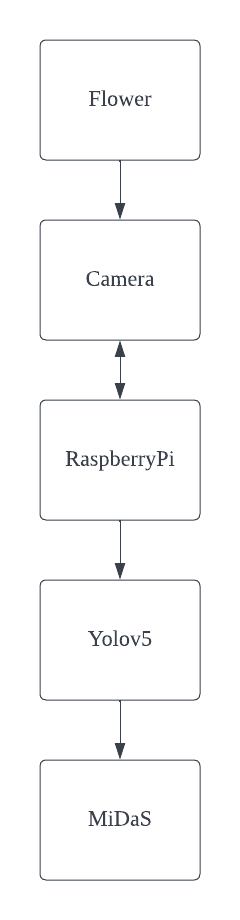
\includegraphics[width=0.1\textwidth]{Figures/Results/Object Detection.png}}
    \caption{Object Detection Flow Chart.}
    \label{fig9}
\end{figure}

Fig. ~\ref{fig9} shows the flowchart of our object detection with the Raspberry Pi embedded system. As you can see the sequence in the flowchart is first using YOLOv5 to detect Flower and then using MiDaS to measure the distance.

\begin{figure}[H]
    \centerline{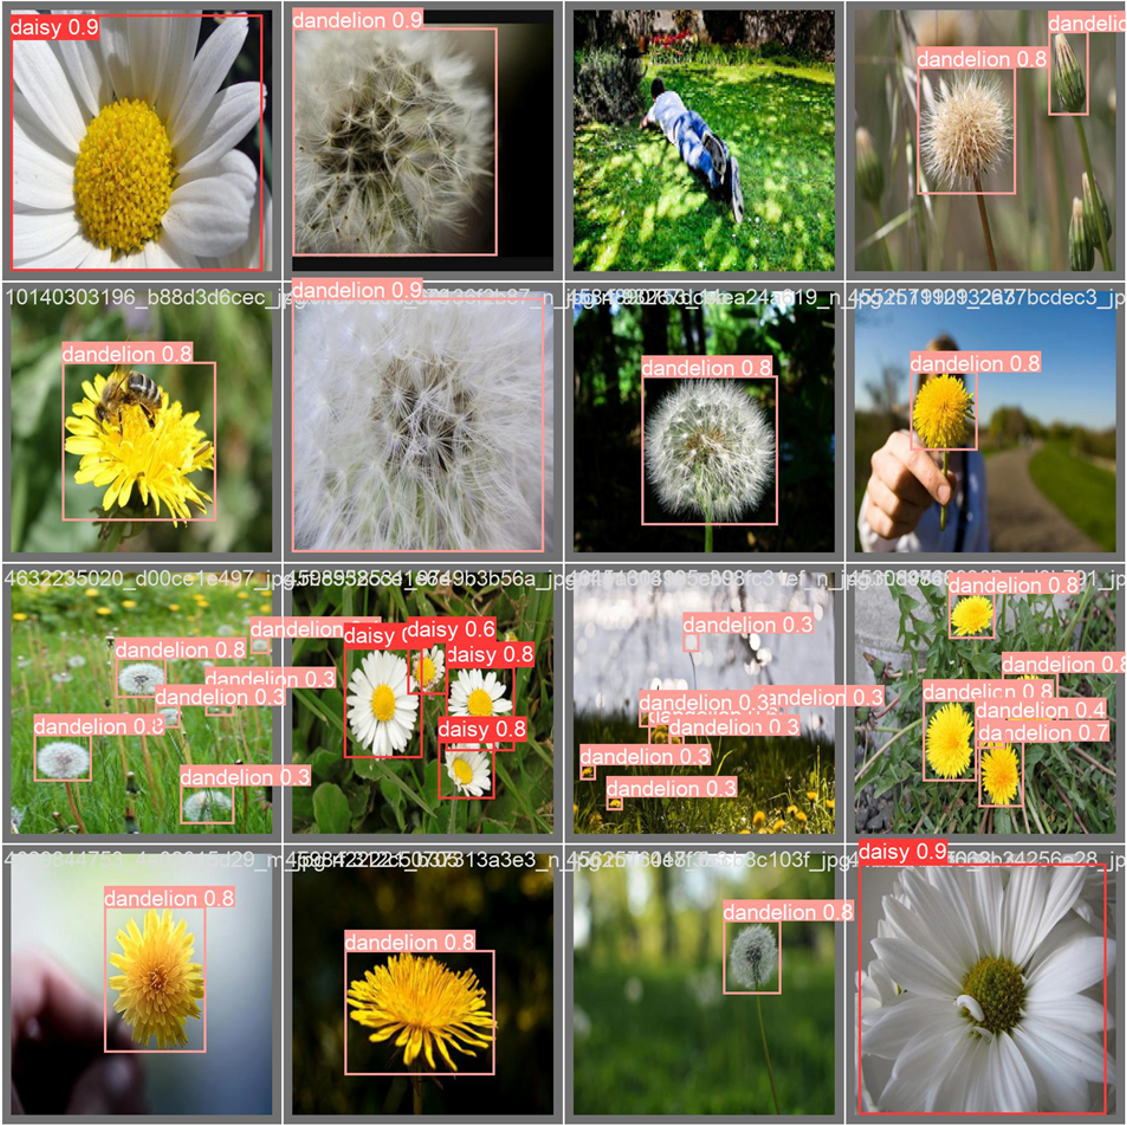
\includegraphics[width=0.5\textwidth]{Figures/Results/RPi_YOLOv5.png}}
    \caption{YOLOv5 model test on real-world dataset with Raspberry Pi 3B.}
    \label{fig10}
\end{figure}

Fig. ~\ref{fig10} shows the results of real-world dataset testing on the Raspberry Pi 3B using the YOLOv5 model. It can be found that the accuracy is considerable, and one of the test images with no flowers on purpose is not misidentified.

As we run Yolov5 on Raspberry Pi 3B, Raspberry Pi 4B, we can clearly see the performance differences among them, as shown in TABLE \ref{tab1}.  
\begin{table}[H]
    \caption{Performance Comparison on running Yolov5}
    \begin{center}
        \resizebox{0.35\textwidth}{!}{%
            \begin{tabular}{|c|c|c|c|}
                \hline
                \textbf{}&\multicolumn{2}{|c|}{\textbf{Controller}} \\
                \cline{2-3} 
                \textbf{Rubric} & \textbf{\textit{RPi3}}& \textbf{\textit{RPi4}} \\
                
                \hline
                CPU (GHz) & 1.2 & 1.5  \\
                \hline
                RAM (GB) & 1 & 8  \\
                \hline
                RAM Usage (MB) & 340 & 332  \\
                \hline
                yolov5s.pt (fps) & 0.21 & 0.95  \\
                \hline
                yolov5n.pt (fps) & 0.43 & 1.67  \\
                \hline
                Load Speed & Very & Very  \\
                (from cmd to start detect) & slow & fast  \\
                
                \hline
            \end{tabular}
        }
        \label{tab1}
    \end{center}
\end{table}

We are also able to control the drone to take off, hover, move in direction, rotation, and landing through Raspberry Pi.

\subsection{Jetson Nano 2GB Integration}

During the integration of the Jetson Nano 2GB and the drone system, we encountered unexpected issues and device malfunctions, which prevented us from incorporating the YOLOv5 detection model and MiDaS depth estimation model into the system. Instead, we utilized the OpenCV library and developed a QR code tracking script that enables the drone to detect QR codes and rotate to track them. 

\begin{figure}[H]
    \centerline{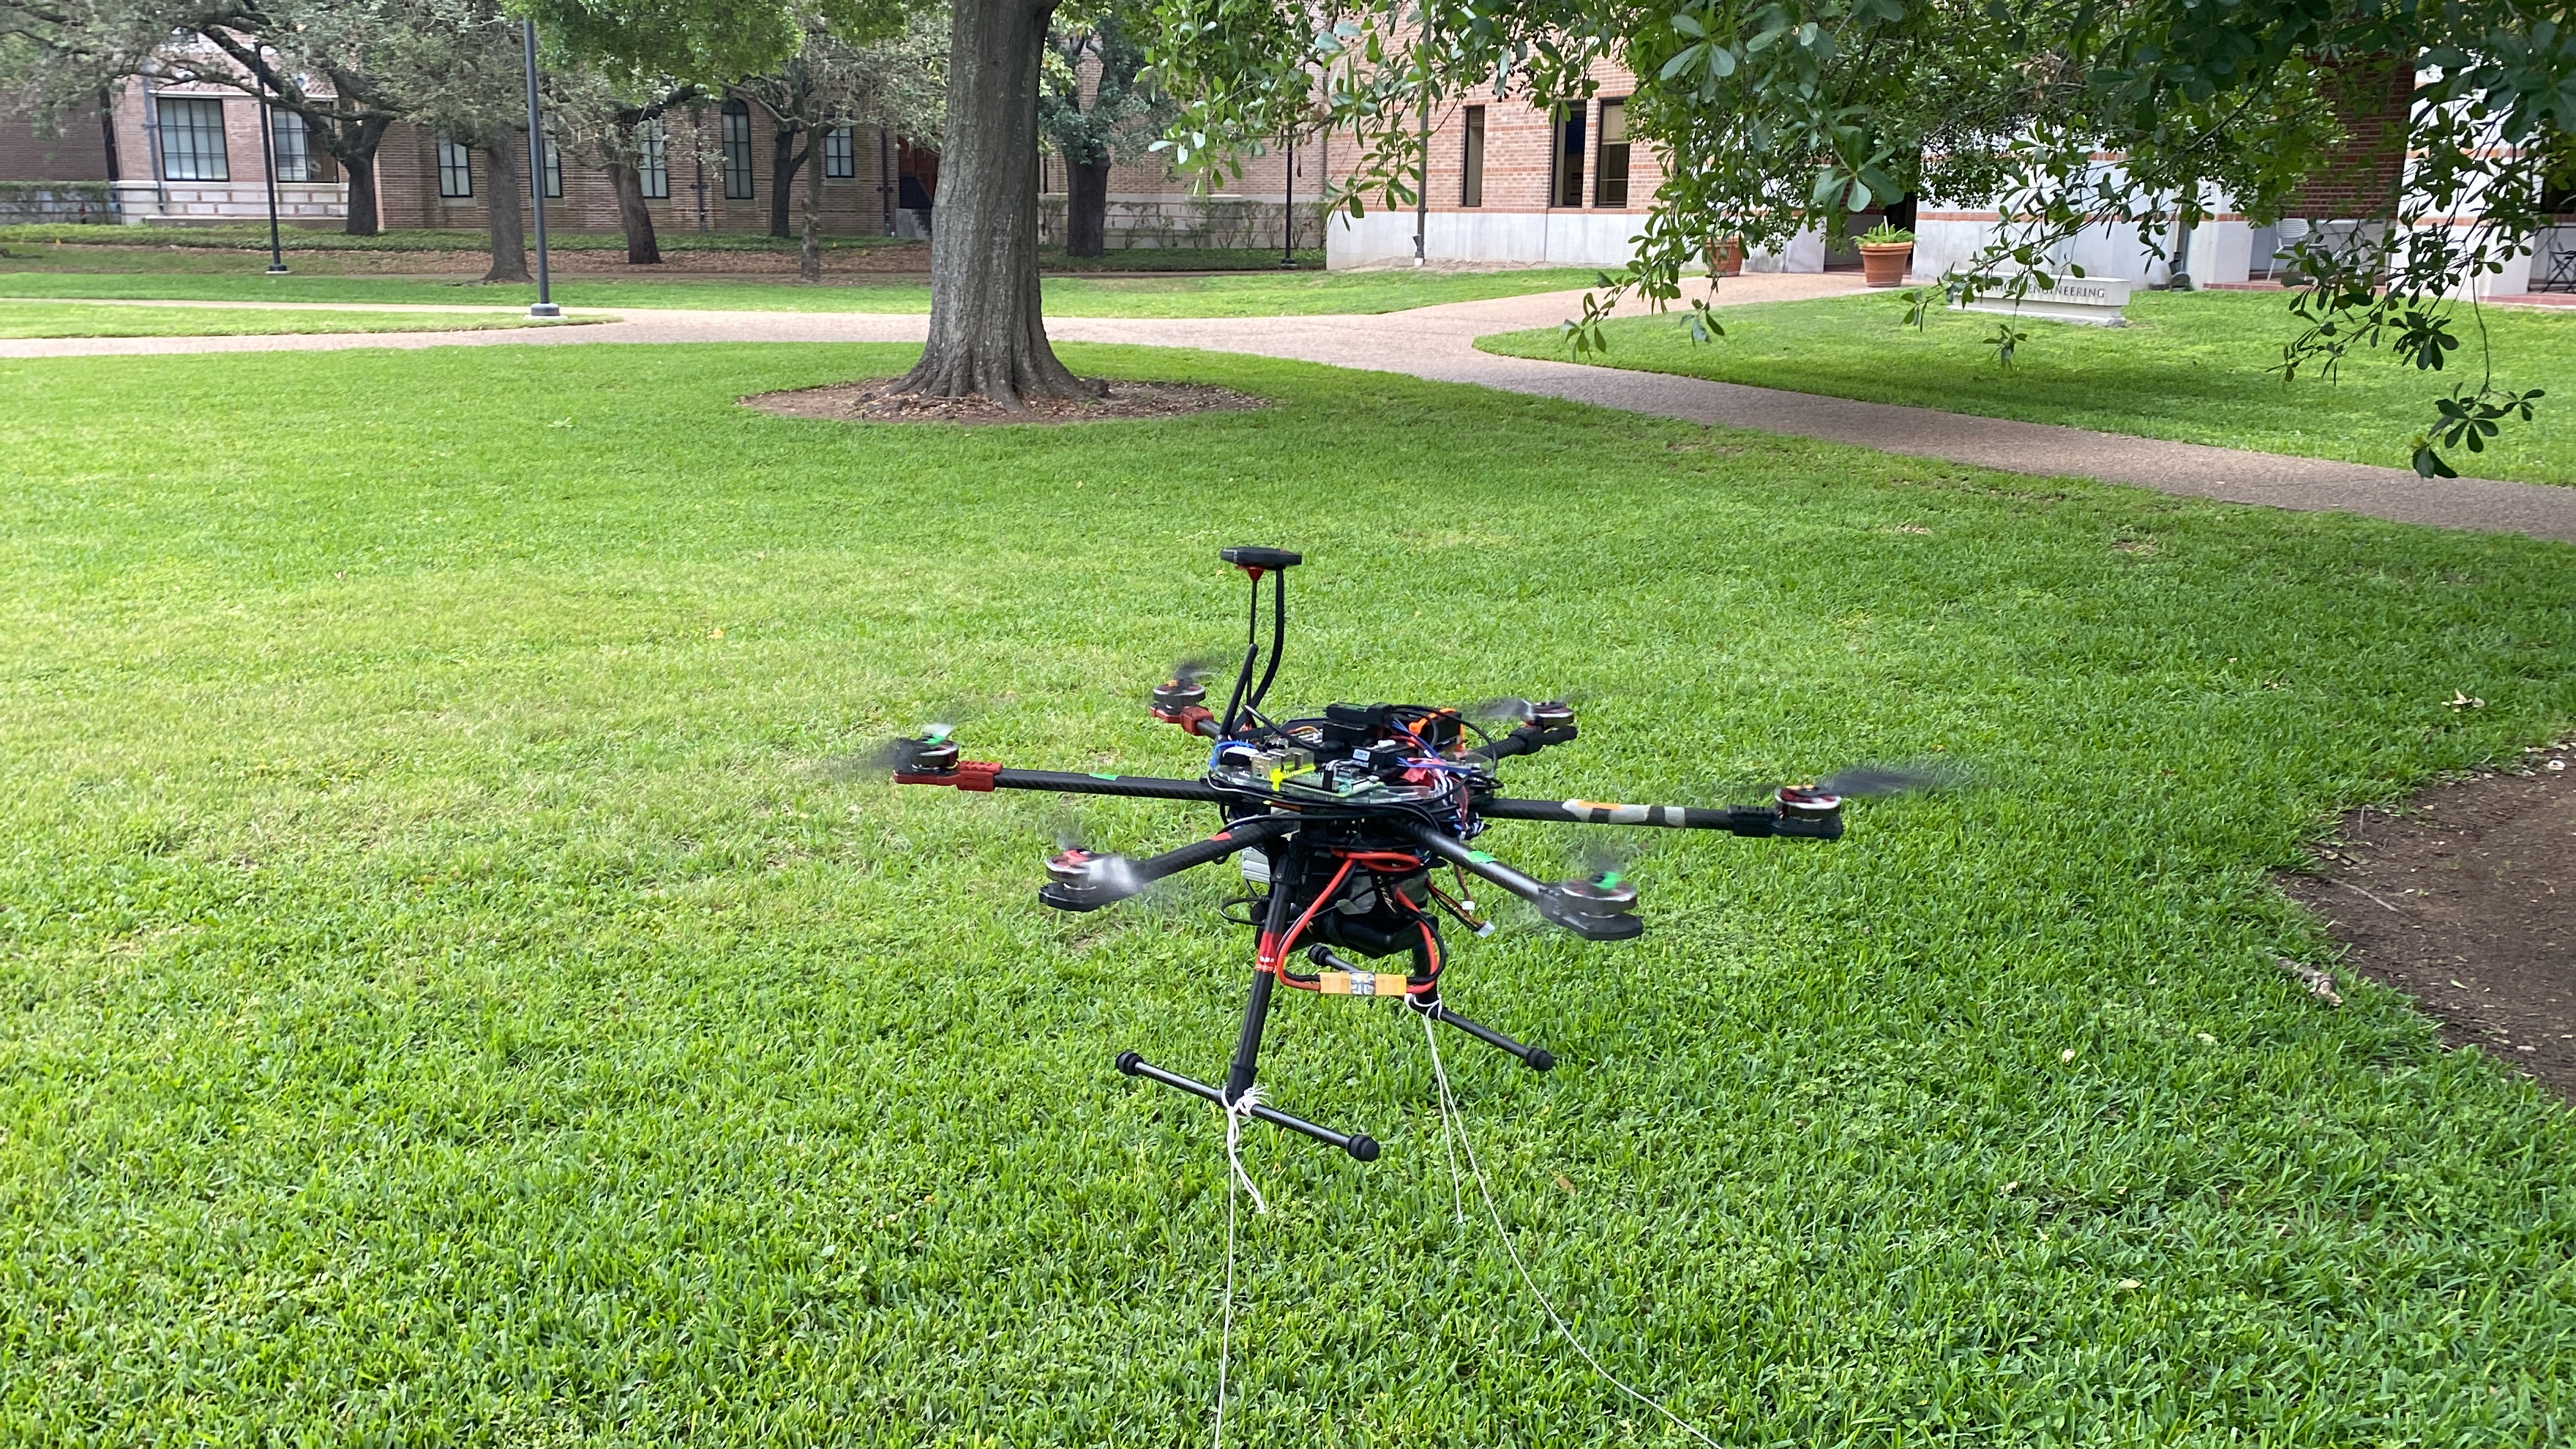
\includegraphics[width=0.5\textwidth]{Figures/Results/Drone_Hover.JPG}}
    \caption{Hover drone in the air operated by Jetson Nano 2GB.}
    \label{fig11}
\end{figure}

Before implementing this experiment, we tested several other simple movement scripts. Fig. ~\ref{fig11} shows the drone hovering successfully in the air for the first time, while Fig. ~\ref{fig12} shows the final experiment in which the drone hovers in the air and tracks the QR code. This experiment was conducted in a real-world environment.

\begin{figure}[H]
    \centerline{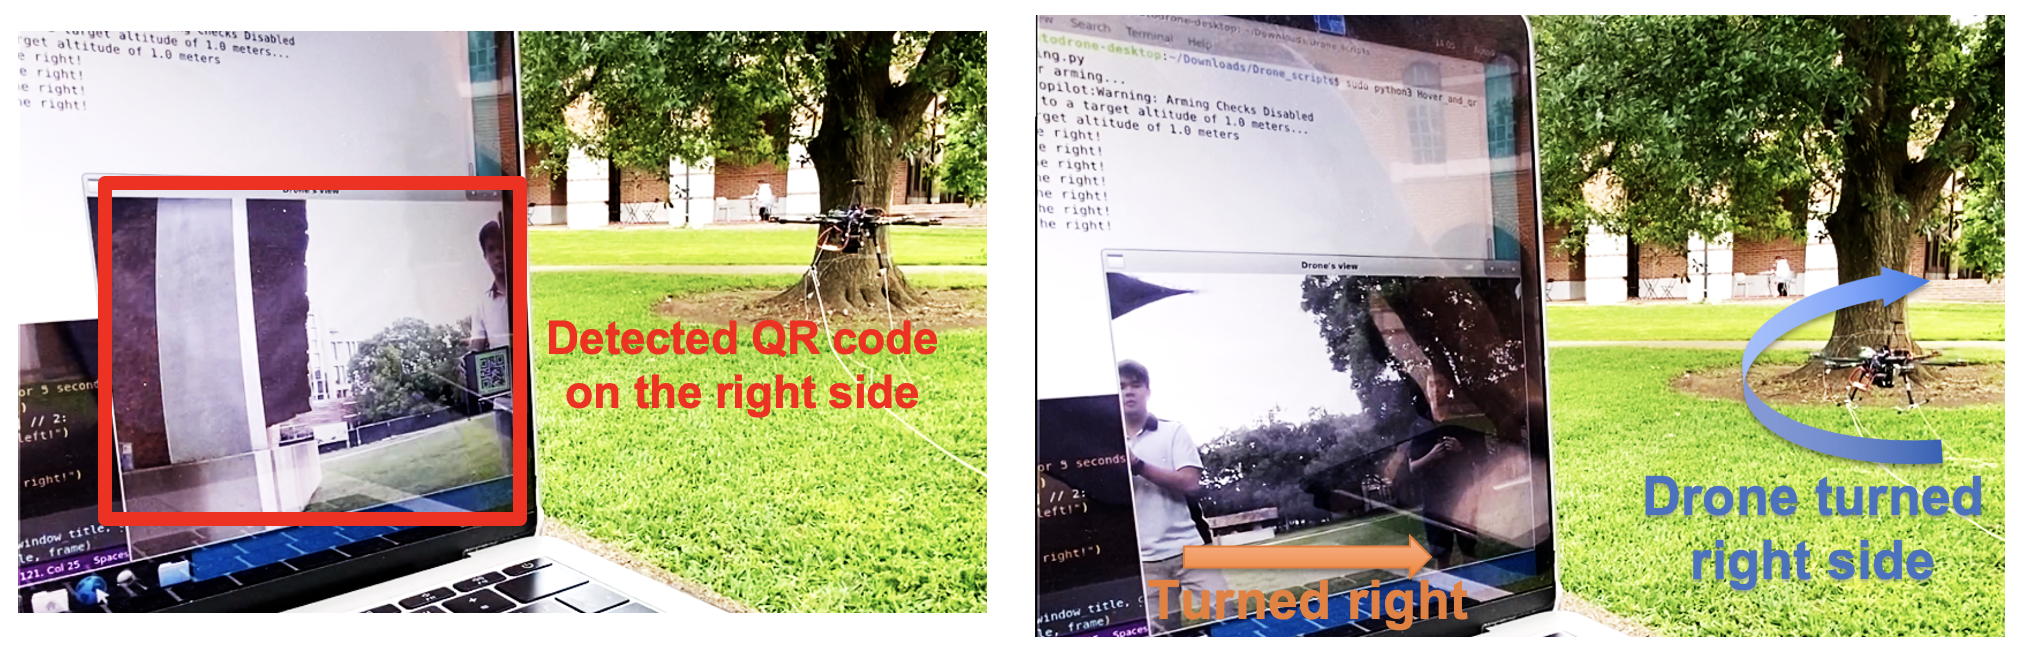
\includegraphics[width=0.5\textwidth]{Figures/Results/QR_code_Tracking_Successfully.png}}
    \caption{QR code tracking results on Jetson Nano 2GB.}
    \label{fig12}
\end{figure}

\subsection{YOLOv5 + MiDaS}

\begin{figure}[H]
    \centerline{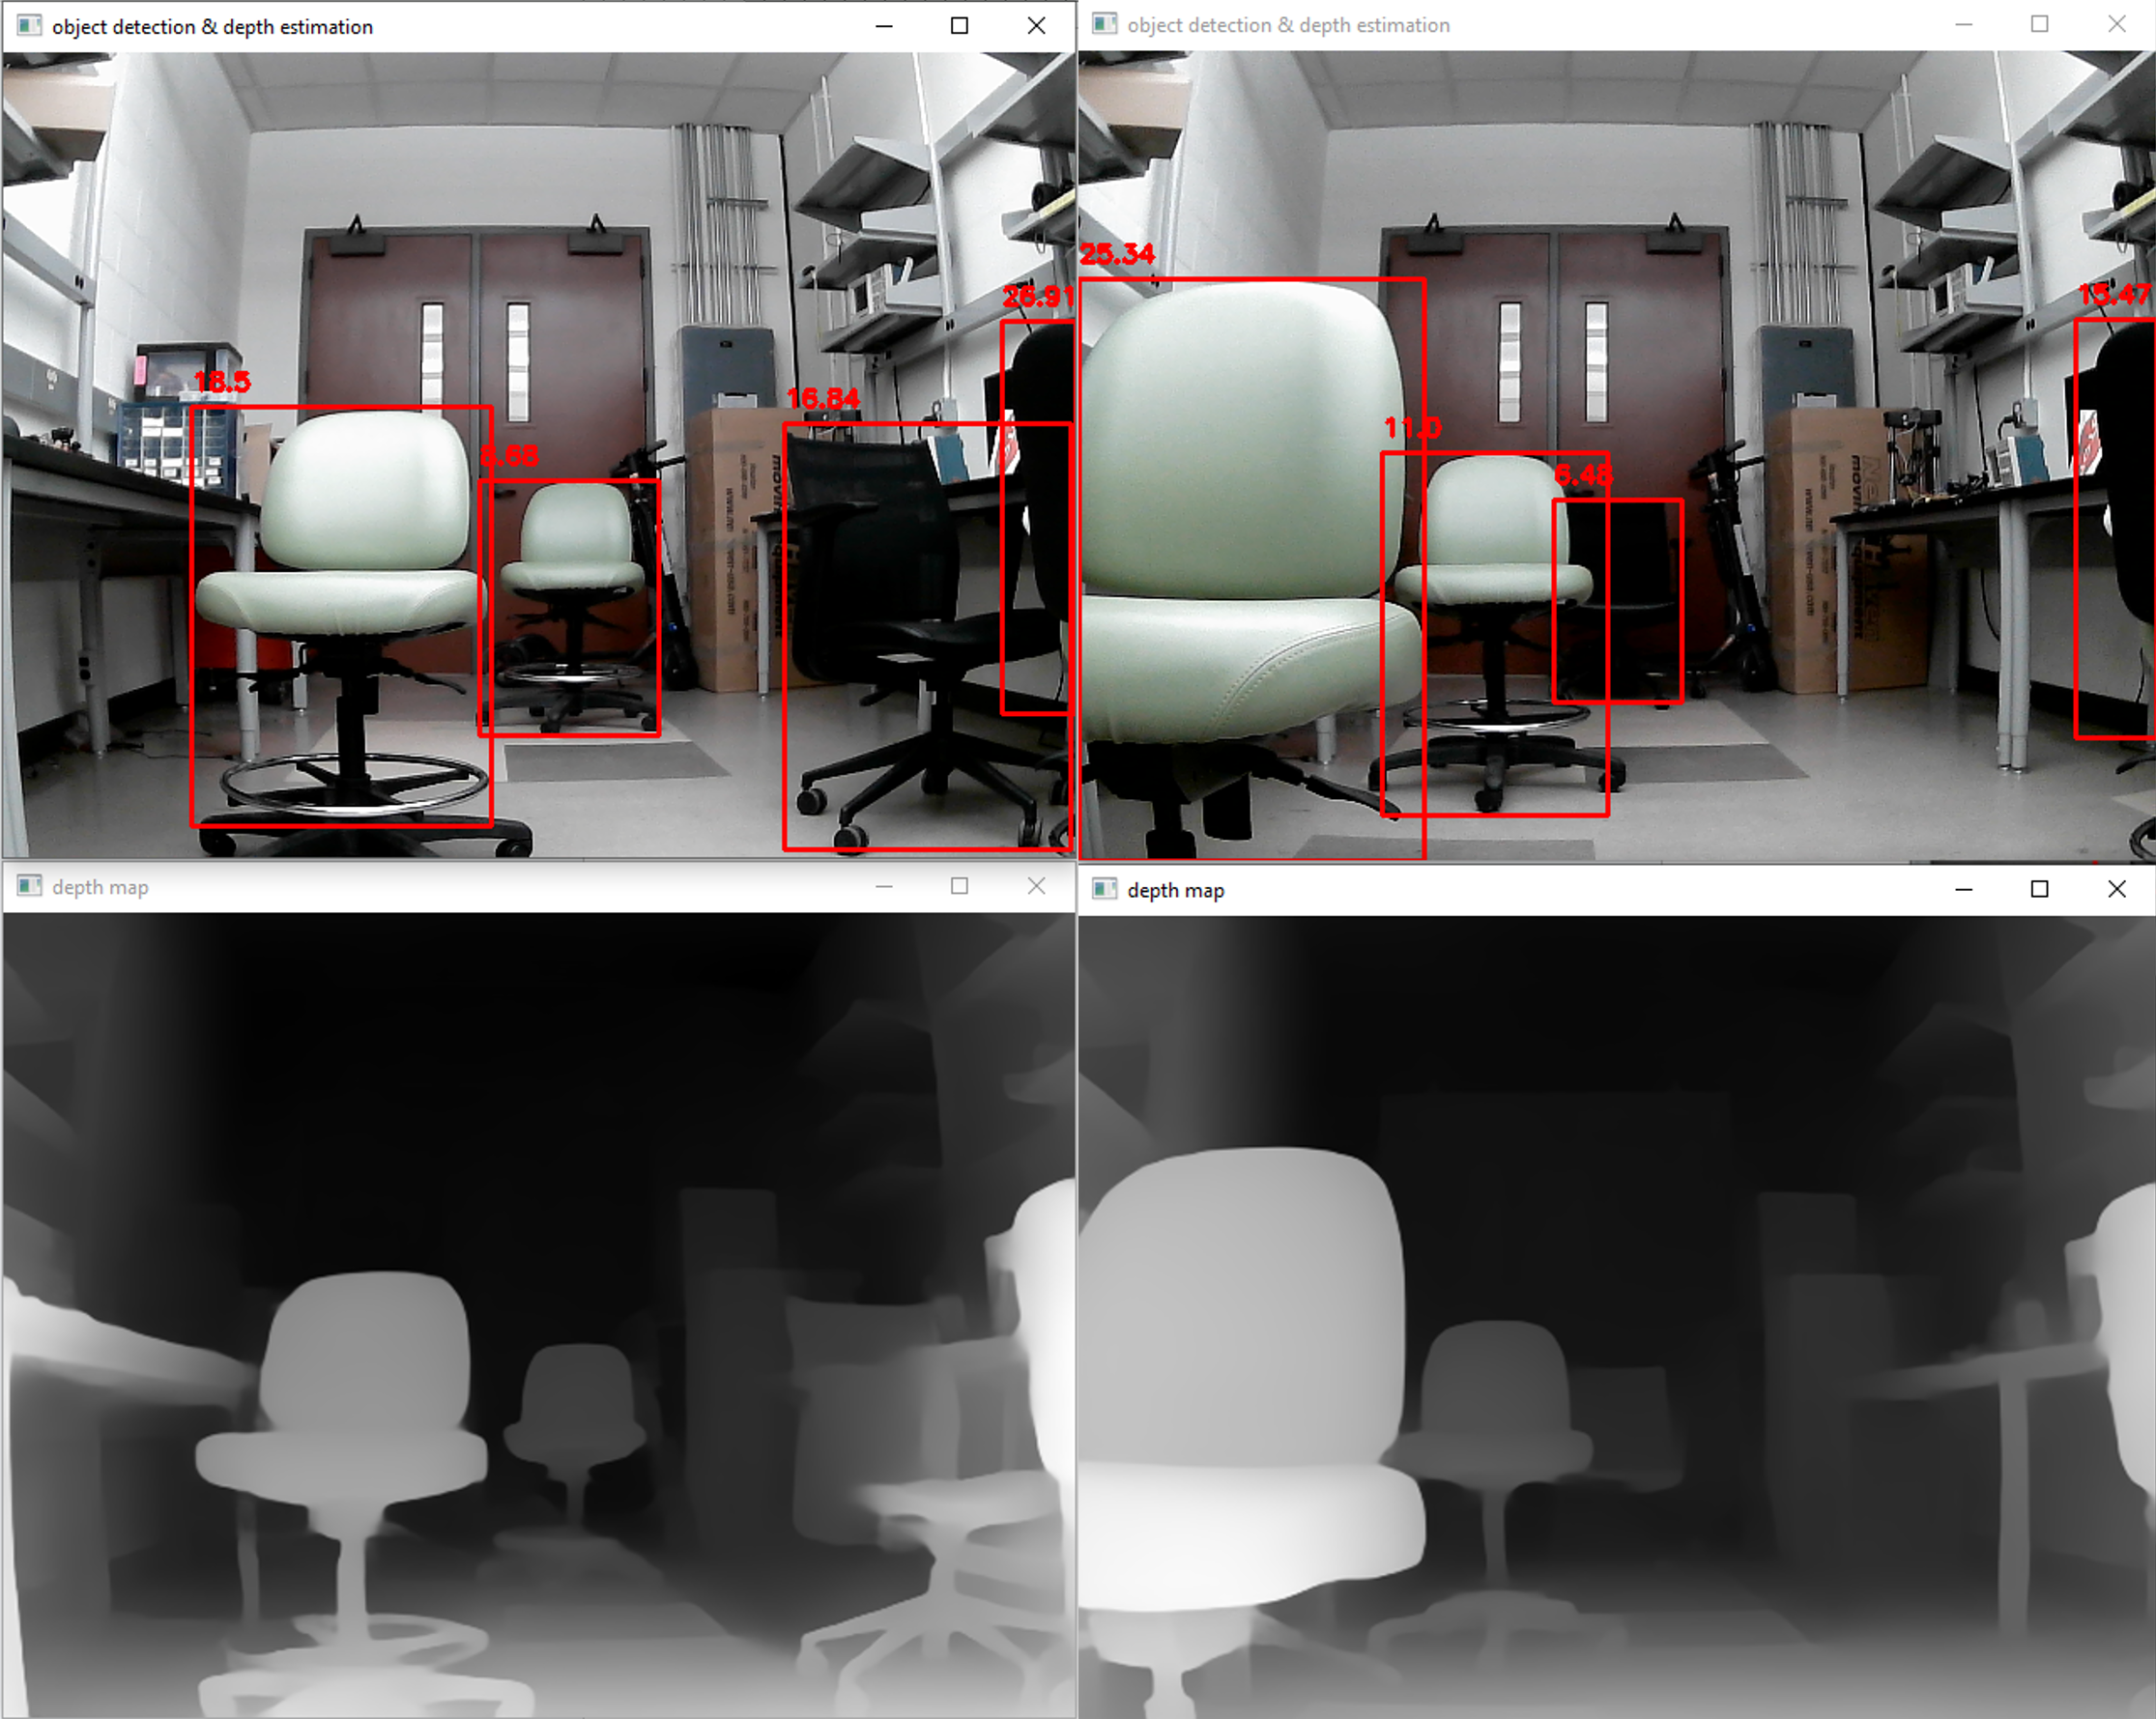
\includegraphics[width=0.5\textwidth]{Figures/Results/exp1.png}}
    \caption{Results of the First Experiment. (top left) YOLOv5 Objects Detected in 2m \& 4m / (top right) YOLOv5 Objects Detected in 1m \& 3m \& 5m / (bottom) Corresponding MiDaS Depth Maps for Visualization}
    \label{fig13}
\end{figure}

\begin{figure}[H]
    \centerline{\includegraphics[width=0.5\textwidth]{Figures/Results/exp2.png}}
    \caption{Results of the Second Experiment. / (top rows) YOLOv5 Objects Detected from the First Orientation in 1m, 2m, 3m, and 3.5 m from Left to Right and Corresponding MiDaS Depth Maps for Visualization / (bottom rows) YOLOv5 Objects Detected from the Second Orientation in 1m, 2m, 3m, and 3.5 m from Left to Right and Corresponding MiDaS Depth Maps for Visualization}
    \label{fig14}
\end{figure}

Fig. ~\ref{fig13} and ~\ref{fig14} display the results of the experiments discussed above. The bounding boxes indicate the objects detected by the YOLOv5 model. The MiDaS model is executed simultaneously, with its depth map displayed at the bottom of each corresponding camera frame. The median intensity of the detected object in the depth map is listed in the top left corner of each bounding box. The depth map intensities and real-world distances of the detected objects in each experiment are listed in Tables ~\ref{tab2} and ~\ref{tab3}, and their relationships are illustrated in Scatter Plots 1 and 2 below.

\begin{table}[H]
    \caption{Data from Experiment 1}
    \begin{center}
        \resizebox{0.45\textwidth}{!}{%
            \begin{tabular}{|c|c|}
                \hline
                \textbf{Real-World Distance (m)}&\textbf{Depth Map Intensity} \\
                \cline{1-2} 
                
                \hline
                1 & 25.34\\
                \hline
                2 & 18.50\\
                \hline
                3 & 11.00\\
                \hline
                4 & 8.68\\
                \hline
                5 & 6.48\\
                \hline
            \end{tabular}
        }
        \label{tab2}
    \end{center}
\end{table}

\pgfplotstableread{
X Y
1 25.34
2 18.50
3 11.00
4 8.68
5 6.48
}\datatable

\begin{figure}[H]
    \centering
    \resizebox{0.45\textwidth}{!}{%
        \begin{tikzpicture}
            \begin{axis}[
                align =center,
                title={Plot 1: Experiment 1 \\ Real-World Distance vs. Depth Map Intensity},
                xlabel={Real-World Distance [m]},
                ylabel={Depth Map Intensity},
                xmin=0, xmax=6,
                ymin=0, ymax=30,
                xtick={0,1,2,3,4,5,6},
                ytick={0,5,10,15,20,25,30}
            ]
        
                \addplot[
                    color=black,
                    only marks,
                    mark=*,
                ]
                table {\datatable};
                % coordinates {
                % (1, 25.34)(2, 18.50)(3, 11.00)(4, 8.68)(5, 6.48)
                % };
                \addplot [thick, red] table[
                    y={create col/linear regression={y=Y}}
                ] % compute a linear regression from the input table
                {\datatable};
            \end{axis}
        \end{tikzpicture}
    }
\end{figure}


\begin{table}[H]
    \caption{Data from Experiment 2}
    \begin{center}
        \resizebox{0.45\textwidth}{!}{%
            \begin{tabular}{|c|c|cc|}
                \hline
                \multirow{2}{*}{} & \multirow{2}{*}{\textbf{Real-World Distance (m)}} & \multicolumn{2}{c|}{\textbf{Depth Map Intensity}} \\ \cline{3-4} 
                                  &                                          & \multicolumn{1}{c|}{Trial 1}  & Trial 2  \\ \hline
                Orien 1           & \multirow{2}{*}{1}                       & \multicolumn{1}{c|}{30.62}    & /        \\ \cline{1-1} \cline{3-4} 
                Orien 2           &                                          & \multicolumn{1}{c|}{28.19}    & 27.15    \\ \hline
                Orien 1           & \multirow{2}{*}{2}                       & \multicolumn{1}{c|}{32.89}    & 32.64    \\ \cline{1-1} \cline{3-4} 
                Orien 2           &                                          & \multicolumn{1}{c|}{32.16}    & 27.78    \\ \hline
                Orien 1           & \multirow{2}{*}{3}                       & \multicolumn{1}{c|}{29.41}    & /        \\ \cline{1-1} \cline{3-4} 
                Orien 2           &                                          & \multicolumn{1}{c|}{28.64}    & /        \\ \hline
                Orien 1           & \multirow{2}{*}{3.5}                     & \multicolumn{1}{c|}{29.44}    & /        \\ \cline{1-1} \cline{3-4} 
                Orien 2           &                                          & \multicolumn{1}{c|}{26.56}    & /        \\ \hline
            \end{tabular}
        }
        \label{tab3}
    \end{center}
\end{table}

\begin{figure}[H]
    \centering
    \resizebox{0.45\textwidth}{!}{%
        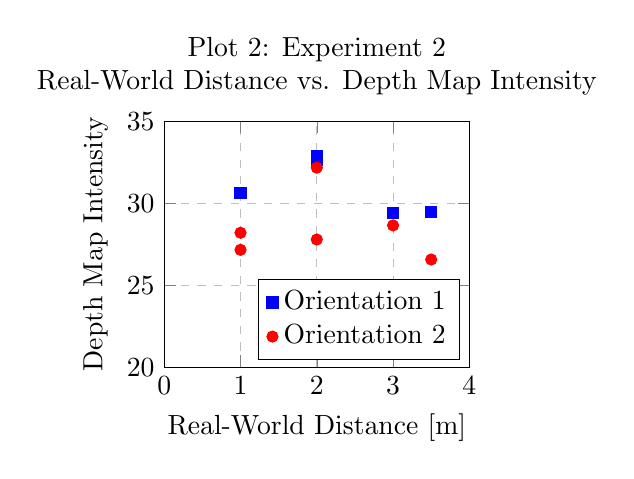
\begin{tikzpicture}
            \begin{axis}[
                align =center,
                title={Plot 2: Experiment 2 \\ Real-World Distance vs. Depth Map Intensity},
                xlabel={Real-World Distance [m]},
                ylabel={Depth Map Intensity},
                xmin=0, xmax=4,
                ymin=20, ymax=35,
                xmajorgrids=true,
                ymajorgrids=true,
                grid style=dashed,
                legend pos=south east
                % xtick={0,1,2,3,4},
                % ytick={20, 23, 26, 29, 32, 35}
            ]
                \addplot[blue,only marks, mark=square*]
                    table[x=x, y=y, col sep=space] {
                    x y
                    1 30.62
                    2 32.89
                    2 32.64
                    3 29.41
                    3.5 29.44
                };
                
                \addplot[red,only marks, mark=*]
                    table[x=x, y=y, col sep=space] {
                    x y
                    1 28.19
                    1 27.15
                    2 32.16
                    2 27.78
                    3 28.64
                    3.5 26.56
                };
                
                \addlegendentry{Orientation 1}
                \addlegendentry{Orientation 2}
            \end{axis}
        \end{tikzpicture}
    }
\end{figure}


In the indoor environment, due to the stable webcam setup and consistent lighting conditions, the scatter plot reveals an approximately linear relationship between the depth map intensity and real-world distance. By determining the slope and intercept of this approximate straight line, we successfully convert a depth map intensity into an approximate real-world distance in the program. The error of this approximation is estimated to be around 10\%.

In the outdoor environment, two observations can be made from the data. Firstly, the object with higher brightness in the first orientation exhibits a higher depth map intensity than the one in the second orientation at the same real-world distance. This discrepancy occurs due to the webcam's auto-exposure adjustment. The orientation of sunlight does affect the depth map intensity, even when objects are positioned at an equal distance from the webcam. Secondly, the depth map intensity varies significantly due to the vibration of the webcam. As the webcam has a fixed focal length and image distance, along with constant vibration on the drone, objects may inevitably appear blurry when they are further away from the camera. From Scatter Plot 2, it is difficult to discern the trend of depth map intensity versus real-world distance. This issue may significantly impact the depth map intensity produced by the MiDaS model, leading to substantial inaccuracies in measurement.

\subsection{UI Interface}

From the system design diagram in Fig.~\ref{fig6}, it can be seen that we connect the Flight Controller to the SIK radio and then to the Mission Planner GUI of the computer, we follow this design to setup on the real drone system, the SIK Telemetry Radio devices on the left side of Fig.~\ref{fig2}, connected one devide to the Cube Black Flight Controller's Telem Port 1, and the other one is connected to the Laptop's USB port, after initializing the settings in Mission Planner, you can successfully see the monitor screen as shown in Fig.~\ref{fig13}.

\begin{figure}[H]
    \centerline{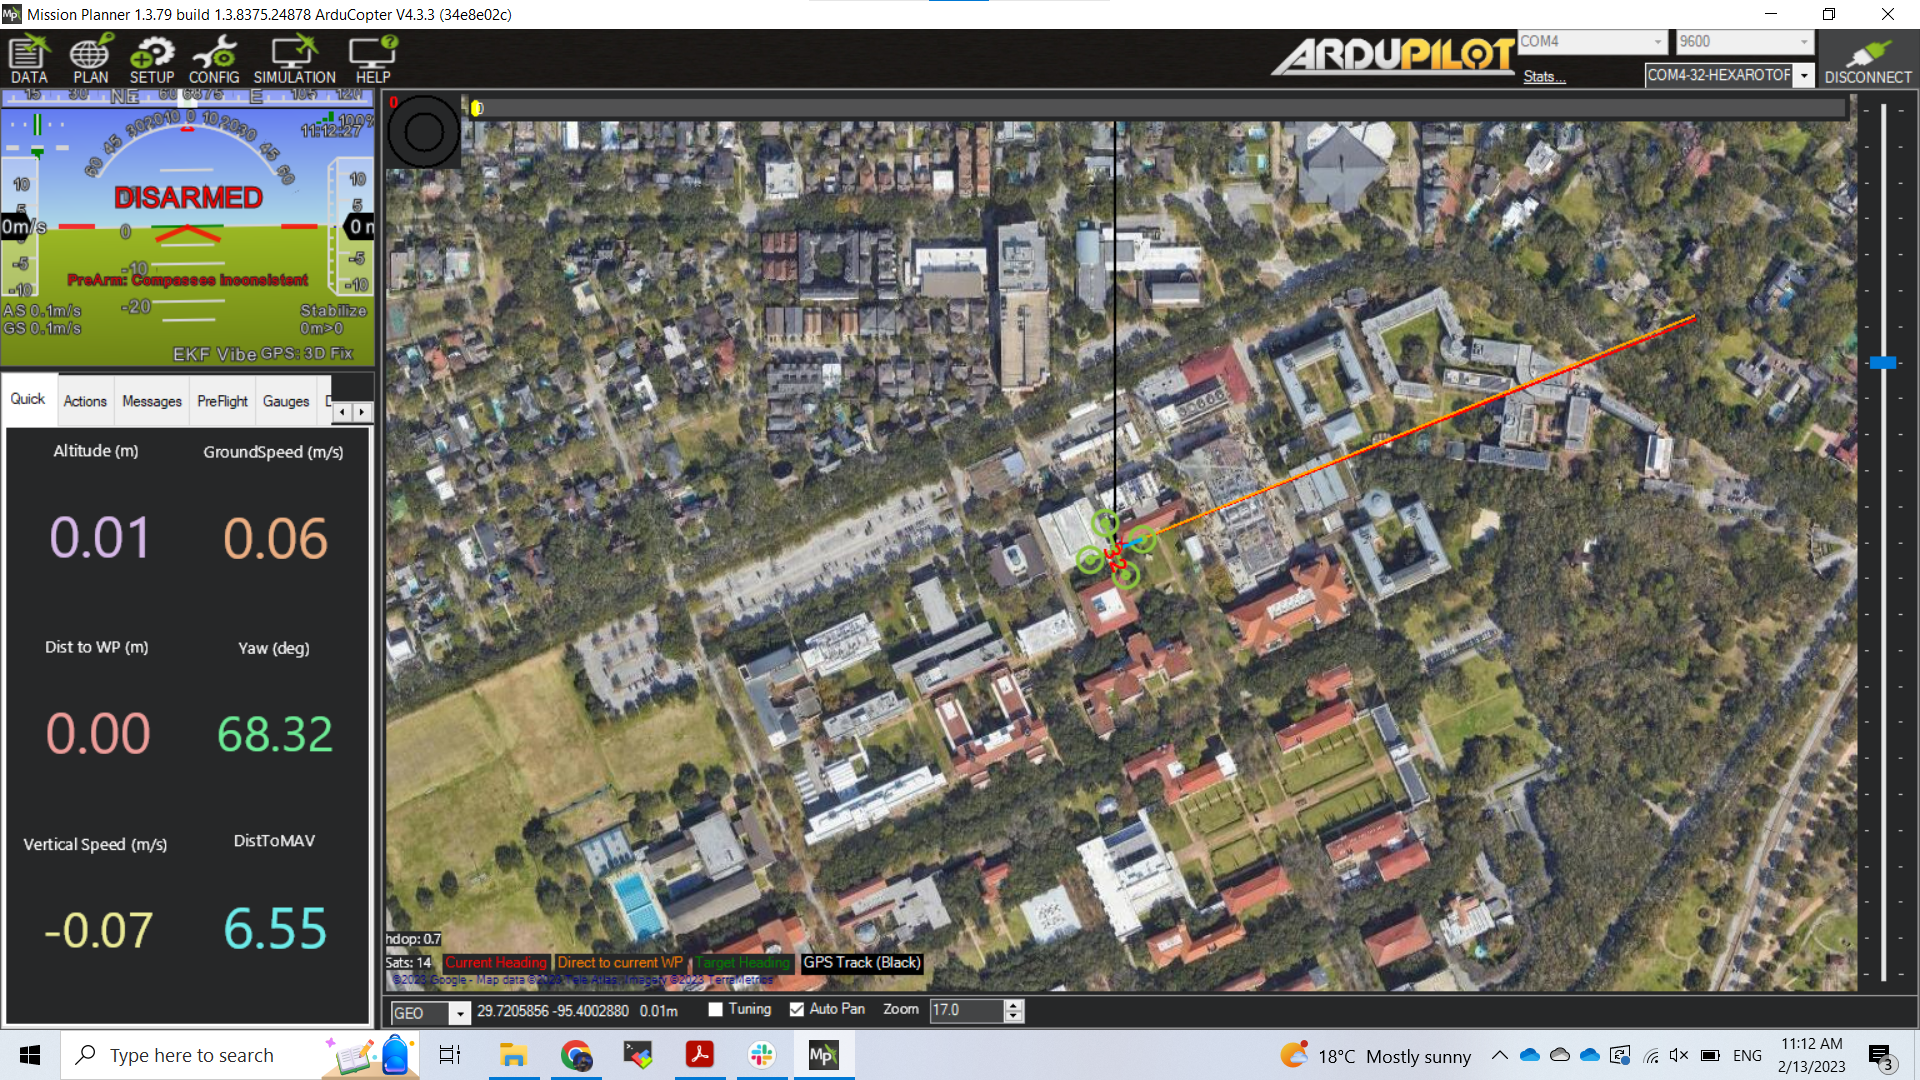
\includegraphics[width=0.5\textwidth]{Figures/Results/Mission_Planner_GUI.png}}
    \caption{Mission Planner GUI Interface.}
    \label{fig15}
\end{figure}

Fig.~\ref{fig14} shows the real-time status of the drone from SIK Telemetry Radio in Mission Planner GUI. The left side of the image shows the "DISARMED" status, which means the drone is not armed yet, and the right picture shows the "ARMED" status, which means the drone is armed and starts to spin the propellers at a fixed speed.

\begin{figure}[H]
    \centerline{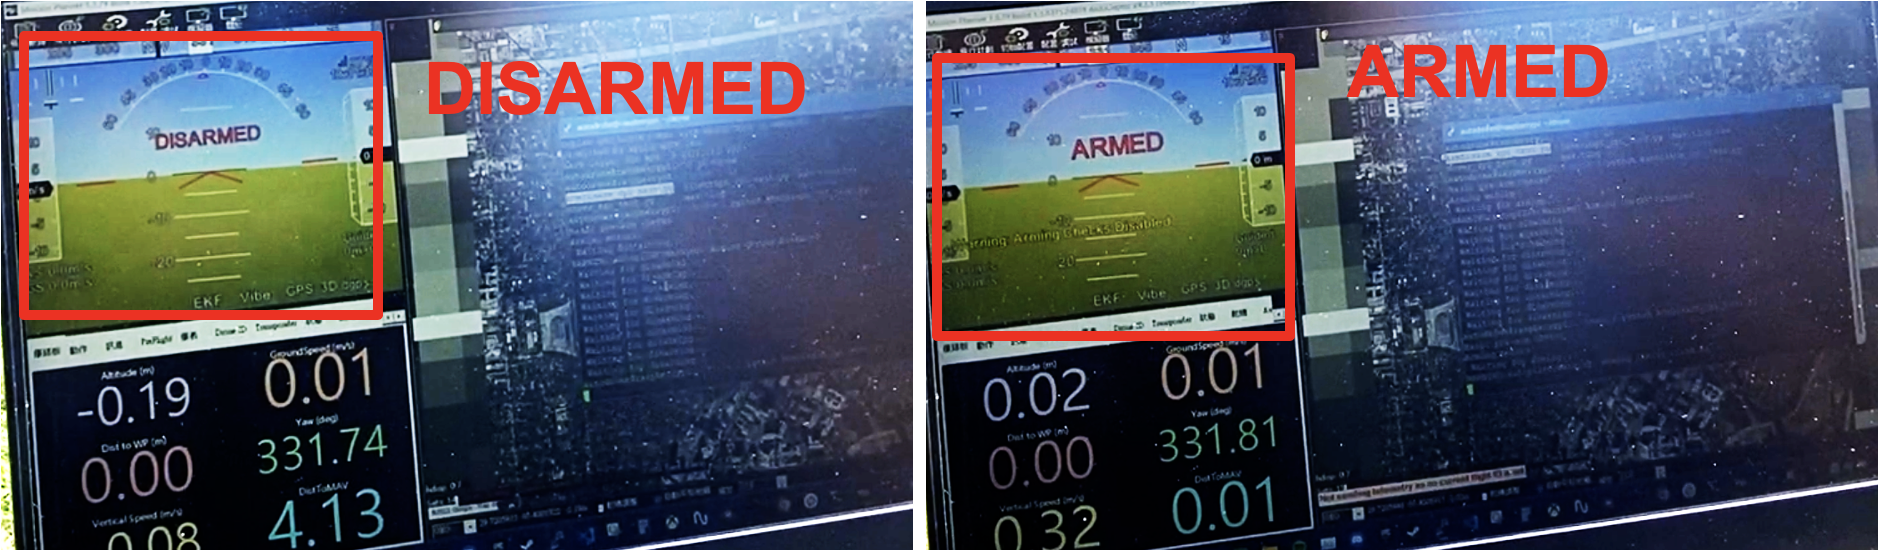
\includegraphics[width=0.5\textwidth]{Figures/Results/GUI_Status.png}}
    \caption{Drone's real-time status on Mission Planner GUI.}
    \label{fig16}
\end{figure}
\section{Discussion}

One of the significant accomplishments in this semester is the successful integration of the QR code tracking script and drone movement script on the Jetson Nano 2GB. The QR code tracking script allowed the drone to detect QR codes and rotate to track them. The drone could also turn right until the QR code was in the center, showing the potential for autonomous navigation using computer vision techniques.

The results from the first MiDaS evaluation experiment reveal that it is reasonably accurate to perform object detection and depth estimation using YOLOv5 and MiDaS models in an indoor environment. However, the outdoor experiment simulating a practical object depth estimation task yields unfavorable results. The depth map intensity is not as accurate as expected and is significantly affected by various factors, such as sunlight orientation, webcam exposure, and drone vibration. Although the MiDaS model is reliable in a stable environment with minimal interference, its application in autonomous drone pollination tasks remains challenging.

These results demonstrate the progress made in the project and pave the way for future developments. In the next semester, we will further research solutions for autonomous drone navigation from the current position to the target position. We will consider either developing a new algorithm utilizing a stereo camera with higher accuracy or exploring alternative methods, such as target and self-localization to determine the relative position first, followed by motion planning. This approach will hopefully enable us to improve the reliability of the autonomous drone navigation system in real-world scenarios.
\section*{Acknowledgment}

Repository for this project are available at: \url{https://github.com/Rice-MECE-Capstone-Projects/Autodrone} \\

Documents and tutorial for this project are available at: \url{https://riceautodrone.github.io/} \\

% \section*{References}

\begin{thebibliography}{00} 
\bibitem{b1} ``United States Honey Bee Colony Losses 2020-2021: Preliminary Results,'' Bee Informed, Jun. 21, 2021, https://beeinformed.org/2021/06/21/united-states-honey-bee-colony-losses-2020-2021-preliminary-results.

\bibitem{b2} ``FAO - News Article: Declining bee populations pose threat to global food security and nutrition,'' Food and Agriculture Organization of the United Nations, May 20, 2019, https://www.fao.org/news/story/en/item/1194910/icode.

\bibitem{b3} K. Ma, P. Chirarattananon, S. Fuller, R. Wood, ``Controlled Flight of a Biologically Inspired, Insect-Scale Robot,'' Science Magazine, vol.340, no. 6132, pp. 603-607, May 2013.

\bibitem{b4} N. Ohi et al., ``Design of an Autonomous Precision Pollination Robot,'' 2018 IEEE/RSJ International Conference on Intelligent Robots and Systems (IROS), 2018, pp. 7711-7718, doi: 10.1109/IROS.2018.8594444.

\bibitem{b5} M. T. Pratama et al., ``Deep Learning-based Object Detection for Crop Monitoring in Soybean Fields,'' 2020 International Joint Conference on Neural Networks (IJCNN), 2020, pp. 1-7, doi: 10.1109/IJCNN48605.2020.9207400.

\bibitem{b6} Z. Sun, X. Guo, Y. Xu, S. Zhang, X. Cheng, Q. Hu, W. Wang, and X. Xue, ``Image recognition of male oilseed rape (brassica napus) plants based on convolutional neural network for UAAS navigation applications on supplementary pollination and aerial spraying,'' Agriculture, vol. 12, no. 1, p. 62, 2022, doi: 10.3390/agriculture12010062. 

\bibitem{b7} J. Redmon, S. Divvala, R. Girshick, A. Farhadi, ``You Only Look Once: Unified, Real-Time Object Detection,'' 2016 IEEE Conference on Computer Vision and Pattern Recognition (CVPR), May 2016, doi: 10.1109/cvpr.2016.91.

\bibitem{b8} G. Jocher et al., ultralytics/yolov5: v6.1 - TensorRT, TensorFlow Edge TPU and OpenVINO Export and Inference (v6.1). Zenodo, 2022, doi: 10.5281/zenodo.6222936.

\bibitem{b9} "Knowledge Distillation." Wikipedia, Wikimedia Foundation, 23 Apr. 2023, en.wikipedia.org/wiki/Knowledge\_distillation. Accessed 24 Apr. 2023.

\bibitem{b10} R. Ranftl, K. Lasinger, D. Hafner, K. Schindler, and V. Koltun, ``Towards Robust Monocular Depth Estimation: Mixing Datasets for Zero-Shot Cross-Dataset Transfer,'' IEEE Transactions on Pattern Analysis and Machine Intelligence, 2019, vol. 44, no. 3, pp. 1623–1637, doi: https://doi.org/10.48550/arXiv.1907.01341

\end{thebibliography}
\vspace{12pt}

%\bibitem{b1} N. Ohi et al., ``Design of an Autonomous Precision Pollination Robot,'' unpublished.
%\bibitem{b2} M. Young, The Technical Writer's Handbook. Mill Valley, CA: University Science, 1989.

% \section{Methods}
Before you begin to format your paper, first write and save the content as a 
separate text file. Complete all content and organizational editing before 
formatting. Please note sections \ref{AA}--\ref{SCM} below for more information on 
proofreading, spelling and grammar.

Keep your text and graphic files separate until after the text has been 
formatted and styled. Do not number text heads---{\LaTeX} will do that 
for you.

\subsection{Abbreviations and Acronyms}\label{AA}
Define abbreviations and acronyms the first time they are used in the text, 
even after they have been defined in the abstract. Abbreviations such as 
IEEE, SI, MKS, CGS, ac, dc, and rms do not have to be defined. Do not use 
abbreviations in the title or heads unless they are unavoidable.

\subsection{Units}
\begin{itemize}
\item Use either SI (MKS) or CGS as primary units. (SI units are encouraged.) English units may be used as secondary units (in parentheses). An exception would be the use of English units as identifiers in trade, such as ``3.5-inch disk drive''.
\item Avoid combining SI and CGS units, such as current in amperes and magnetic field in oersteds. This often leads to confusion because equations do not balance dimensionally. If you must use mixed units, clearly state the units for each quantity that you use in an equation.
\item Do not mix complete spellings and abbreviations of units: ``Wb/m\textsuperscript{2}'' or ``webers per square meter'', not ``webers/m\textsuperscript{2}''. Spell out units when they appear in text: ``. . . a few henries'', not ``. . . a few H''.
\item Use a zero before decimal points: ``0.25'', not ``.25''. Use ``cm\textsuperscript{3}'', not ``cc''.)
\end{itemize}

\subsection{Equations}
Number equations consecutively. To make your 
equations more compact, you may use the solidus (~/~), the exp function, or 
appropriate exponents. Italicize Roman symbols for quantities and variables, 
but not Greek symbols. Use a long dash rather than a hyphen for a minus 
sign. Punctuate equations with commas or periods when they are part of a 
sentence, as in:
\begin{equation}
a+b=\gamma\label{eq}
\end{equation}

Be sure that the 
symbols in your equation have been defined before or immediately following 
the equation. Use ``\eqref{eq}'', not ``Eq.~\eqref{eq}'' or ``equation \eqref{eq}'', except at 
the beginning of a sentence: ``Equation \eqref{eq} is . . .''

\subsection{\LaTeX-Specific Advice}

Please use ``soft'' (e.g., \verb|\eqref{Eq}|) cross references instead
of ``hard'' references (e.g., \verb|(1)|). That will make it possible
to combine sections, add equations, or change the order of figures or
citations without having to go through the file line by line.

Please don't use the \verb|{eqnarray}| equation environment. Use
\verb|{align}| or \verb|{IEEEeqnarray}| instead. The \verb|{eqnarray}|
environment leaves unsightly spaces around relation symbols.

Please note that the \verb|{subequations}| environment in {\LaTeX}
will increment the main equation counter even when there are no
equation numbers displayed. If you forget that, you might write an
article in which the equation numbers skip from (17) to (20), causing
the copy editors to wonder if you've discovered a new method of
counting.

{\BibTeX} does not work by magic. It doesn't get the bibliographic
data from thin air but from .bib files. If you use {\BibTeX} to produce a
bibliography you must send the .bib files. 

{\LaTeX} can't read your mind. If you assign the same label to a
subsubsection and a table, you might find that Table I has been cross
referenced as Table IV-B3. 

{\LaTeX} does not have precognitive abilities. If you put a
\verb|\label| command before the command that updates the counter it's
supposed to be using, the label will pick up the last counter to be
cross referenced instead. In particular, a \verb|\label| command
should not go before the caption of a figure or a table.

Do not use \verb|\nonumber| inside the \verb|{array}| environment. It
will not stop equation numbers inside \verb|{array}| (there won't be
any anyway) and it might stop a wanted equation number in the
surrounding equation.

\subsection{Some Common Mistakes}\label{SCM}
\begin{itemize}
\item The word ``data'' is plural, not singular.
\item The subscript for the permeability of vacuum $\mu_{0}$, and other common scientific constants, is zero with subscript formatting, not a lowercase letter ``o''.
\item In American English, commas, semicolons, periods, question and exclamation marks are located within quotation marks only when a complete thought or name is cited, such as a title or full quotation. When quotation marks are used, instead of a bold or italic typeface, to highlight a word or phrase, punctuation should appear outside of the quotation marks. A parenthetical phrase or statement at the end of a sentence is punctuated outside of the closing parenthesis (like this). (A parenthetical sentence is punctuated within the parentheses.)
\item A graph within a graph is an ``inset'', not an ``insert''. The word alternatively is preferred to the word ``alternately'' (unless you really mean something that alternates).
\item Do not use the word ``essentially'' to mean ``approximately'' or ``effectively''.
\item In your paper title, if the words ``that uses'' can accurately replace the word ``using'', capitalize the ``u''; if not, keep using lower-cased.
\item Be aware of the different meanings of the homophones ``affect'' and ``effect'', ``complement'' and ``compliment'', ``discreet'' and ``discrete'', ``principal'' and ``principle''.
\item Do not confuse ``imply'' and ``infer''.
\item The prefix ``non'' is not a word; it should be joined to the word it modifies, usually without a hyphen.
\item There is no period after the ``et'' in the Latin abbreviation ``et al.''.
\item The abbreviation ``i.e.'' means ``that is'', and the abbreviation ``e.g.'' means ``for example''.
\end{itemize}
An excellent style manual for science writers is \cite{b7}.

\subsection{Authors and Affiliations}
\textbf{The class file is designed for, but not limited to, six authors.} A 
minimum of one author is required for all conference articles. Author names 
should be listed starting from left to right and then moving down to the 
next line. This is the author sequence that will be used in future citations 
and by indexing services. Names should not be listed in columns nor group by 
affiliation. Please keep your affiliations as succinct as possible (for 
example, do not differentiate among departments of the same organization).

\subsection{Identify the Headings}
Headings, or heads, are organizational devices that guide the reader through 
your paper. There are two types: component heads and text heads.

Component heads identify the different components of your paper and are not 
topically subordinate to each other. Examples include Acknowledgments and 
References and, for these, the correct style to use is ``Heading 5''. Use 
``figure caption'' for your Figure captions, and ``table head'' for your 
table title. Run-in heads, such as ``Abstract'', will require you to apply a 
style (in this case, italic) in addition to the style provided by the drop 
down menu to differentiate the head from the text.

Text heads organize the topics on a relational, hierarchical basis. For 
example, the paper title is the primary text head because all subsequent 
material relates and elaborates on this one topic. If there are two or more 
sub-topics, the next level head (uppercase Roman numerals) should be used 
and, conversely, if there are not at least two sub-topics, then no subheads 
should be introduced.

\subsection{Figures and Tables}
\paragraph{Positioning Figures and Tables} Place figures and tables at the top and 
bottom of columns. Avoid placing them in the middle of columns. Large 
figures and tables may span across both columns. Figure captions should be 
below the figures; table heads should appear above the tables. Insert 
figures and tables after they are cited in the text. Use the abbreviation 
``Fig.~\ref{fig}'', even at the beginning of a sentence.

\begin{table}[htbp]
\caption{Table Type Styles}
\begin{center}
\begin{tabular}{|c|c|c|c|}
\hline
\textbf{Table}&\multicolumn{3}{|c|}{\textbf{Table Column Head}} \\
\cline{2-4} 
\textbf{Head} & \textbf{\textit{Table column subhead}}& \textbf{\textit{Subhead}}& \textbf{\textit{Subhead}} \\
\hline
copy& More table copy$^{\mathrm{a}}$& &  \\
\hline
\multicolumn{4}{l}{$^{\mathrm{a}}$Sample of a Table footnote.}
\end{tabular}
\label{tab1}
\end{center}
\end{table}

\begin{figure}[htbp]
\centerline{
\includegraphics{fig1.png}}
\caption{Example of a figure caption.}
\label{fig}
\end{figure}

Figure Labels: Use 8 point Times New Roman for Figure labels. Use words 
rather than symbols or abbreviations when writing Figure axis labels to 
avoid confusing the reader. As an example, write the quantity 
``Magnetization'', or ``Magnetization, M'', not just ``M''. If including 
units in the label, present them within parentheses. Do not label axes only 
with units. In the example, write ``Magnetization (A/m)'' or ``Magnetization 
\{A[m(1)]\}'', not just ``A/m''. Do not label axes with a ratio of 
quantities and units. For example, write ``Temperature (K)'', not 
``Temperature/K''.


\end{document}
